\documentclass[a4paper, 12pt, english]{article}

% \usepackage[portuges]{babel}
\usepackage[utf8]{inputenc}
\usepackage{amsmath,amssymb}
\usepackage{graphicx}
\usepackage{subfig}
\usepackage[colorinlistoftodos]{todonotes}

\usepackage{indentfirst}
\usepackage{verbatim}
\usepackage{textcomp}
\usepackage{gensymb}

\usepackage{relsize}

\usepackage{lipsum}% http://ctan.org/pkg/lipsum
\usepackage{xcolor}% http://ctan.org/pkg/xcolor
\usepackage{xparse}% http://ctan.org/pkg/xparse
\NewDocumentCommand{\myrule}{O{1pt} O{2pt} O{black}}{%
  \par\nobreak % don't break a page here
  \kern\the\prevdepth % don't take into account the depth of the preceding line
  \kern#2 % space before the rule
  {\color{#3}\hrule height #1 width\hsize} % the rule
  \kern#2 % space after the rule
  \nointerlineskip % no additional space after the rule
}
\usepackage[section]{placeins}

\usepackage{booktabs}
\usepackage{colortbl}%
   \newcommand{\myrowcolour}{\rowcolor[gray]{0.925}}
   
\usepackage[obeyspaces]{url}
\usepackage{etoolbox}
\usepackage[colorlinks,citecolor=black,urlcolor=blue,bookmarks=false,hypertexnames=true]{hyperref} 

\usepackage{geometry}
\geometry{
	paper=a4paper, % Change to letterpaper for US letter
	inner=3cm, % Inner margin
	outer=3cm, % Outer margin
	bindingoffset=.5cm, % Binding offset
	top=2cm, % Top margin
	bottom=2cm, % Bottom margin
	%showframe, % Uncomment to show how the type block is set on the page
}
%*******************************************************************************%
%************************************START**************************************%
%*******************************************************************************%
\begin{document}

\begin{titlepage}
\begin{center}
\vspace*{2cm} % Shifts everything down by 2 cm
% Optional Logo or Image
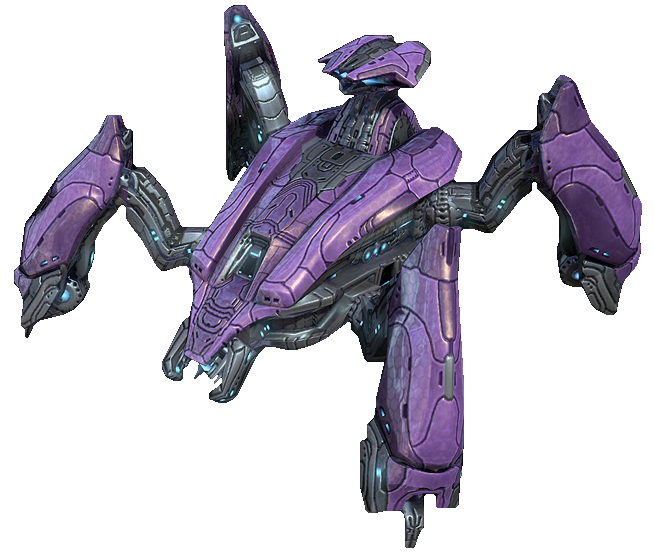
\includegraphics[width=0.3\textwidth]{scarab.png} \\[1cm] % Replace with your logo file path
\newcommand{\HRule}[1]{\rule{\linewidth}{#1}} % Custom horizontal rule
% Title
\HRule{2pt} \\[0.5cm]
\textbf{\LARGE Optimizing Resource Strategies   \\[0.2cm] 
Through Simulation and Iterative  \\[0.3cm]
Analysis in the Halo Wars \\[0.3cm]
Virtual Economy} \\[0.5cm]
\HRule{2pt} \\[1cm]



% Author Name
\textbf{\large Joel Yuhas} \\[1cm]

% Optional Institution
\textbf{\large Independent Research} \\[0.5cm]

% Date
\textbf{\large \today} \\[2cm]

\textit{A computational approach to identifying and optimizing the fastest build strategies in the Halo Wars virtual economy, focusing on resource efficiency and problem solving using Python.}

\vfill

\end{center}
\end{titlepage}





%********************************%
%***********SECTION 1************%
%********************************%
\newpage
\section{Abstract}
This project investigates the optimization of resource collection and build strategies in the real-time strategy game Halo Wars, focusing on constructing the Scarab unit as efficiently as possible. A Python-based simulator was developed to model the game’s economy, incorporating randomized build order generation and validation mechanisms to explore different build combinations. Through extensive testing, the system accurately predicted resource values and identified build orders achieving resource thresholds up to 28\% faster than previous manual strategies. These results validate the effectiveness of computational methods in strategy optimization, providing valuable insights for players and developers alike.

\newpage
% Table of Contents
\tableofcontents
\newpage

\section{Introduction}
Halo Wars, a real-time strategy video game released in 2009, challenges players to manage bases, armies, and resources in order to defeat their opponents. Central to the game is an intricate economy system, where players must carefully balance resource production, technological upgrades, and unit creation to gain an edge. Mastering this economy requires strategic decisions about which buildings to construct, when to upgrade, and how to sequence actions for maximum efficiency.
\newline

One of the most powerful units in Halo Wars is the Scarab—a Super Unit that requires substantial resources and a high technological level to build. Identifying the fastest way to construct a Scarab can provide players with a significant advantage, enabling them to deploy an extremely powerful unit earlier than their opponents. However, the open-ended nature of the game, combined with numerous variables like build order and resource collection rates, makes finding the optimal strategy a complex and time-consuming problem.
\newline

This project aims to address that challenge by leveraging computational simulation to analyze and optimize build orders that effect the players in-game economy. Using Python, a simulator was developed to model the game’s economy with high accuracy, enabling the evaluation of various build order strategies. By iterating through randomly generated and verified build orders, the program can be used to identify the fastest sequences to achieve specific resource thresholds, such as the 3000 resources required to build a Scarab.
\newline

The primary goal of this research was to discover a build order faster than the current personal best of 430 seconds (7 minutes and 10 seconds). Additionally, the project sought to explore advanced coding techniques, create a scalable simulation framework, and validate the findings through real-world gameplay. A stretch goal included determining the fastest way to build two Scarabs, a scenario requiring even greater optimization.
\newline

Ultimately, this work offers insights not only into Halo Wars strategies but also into the broader potential of computational methods for solving optimization problems in games and beyond. The results showcase the effectiveness of combining simulation and iterative analysis to tackle complex strategic challenges, laying the groundwork for further exploration and applications.
\newline

%********************************%
%***********SECTION 2************%
%********************************%

\newpage
\section{Objectives}
\begin{enumerate}
    \item \textbf{Primary Goal}:
    \begin{itemize}
        \item Use Python to discover the fastest way to build a Scarab Super Unit in Halo Wars, optimizing resource efficiency and minimizing build time.
    \end{itemize}

    \item \textbf{Performance Benchmark}:
    \begin{itemize}
        \item Attempt to surpass the personal best time of 7 minutes and 10 seconds (430 seconds) to reach 3000 resources required to start construction on the Scarab.
    \end{itemize}

    \item \textbf{Assumptions}:
    \begin{itemize}
        \item Simulate ideal gameplay conditions, including the specific advantages of the "Exile" map (e.g., access to free tech levels and uncontested second base slots). More information in the Assumptions section.
    \end{itemize}

    \item \textbf{Exploration of Stretch Goals}:
    \begin{itemize}
        \item Investigate strategies to build two Scarabs, requiring 6800 resources and additional upgrades, under similar optimization constraints.
    \end{itemize}

    \item \textbf{Skill Development}:
    \begin{itemize}
        \item Utilize the project as a learning opportunity to practice advanced software development techniques and problem-solving in Python.
    \end{itemize}

    \item \textbf{Validation}:
    \begin{itemize}
        \item Test and validate the simulator's results against actual in-game performance to ensure accuracy and practical applicability.
    \end{itemize}
\end{enumerate}


        
\section{Problem Definition}

		

\subsection{Game Background}
A "Scarab" is the most powerful Super Unit in the game, and also the most expensive. The motivation for finding an answer to the primary objective above is that if a player can produce the strongest unit as fast as possible, it can provide them a massive advantage against their opponents. To optimize the build process for the Scarab, it’s essential to first define its specific prerequisites and the game mechanics governing its production. 
\newline

Halo wars has two factions the player can play as, the "UNSC" and the "Covenant", each with their own unique abilities and special units. The Scarab is only available to the Covenant faction, and thus the player must play as the Covenant.
\newline

To build a Scarab, a player must produce enough resources (3000) and acquire a high enough Technology level (Tech level of 3).
The player gains resources by creating and upgrading buildings called "Supply Pads" on their base. These buildings and upgrades cost resources to construct, but provide the player with a steady stream of resources over time after they're built. 
\newline

The player also has a "Technology" level, which for the Covenant ranges from zero to three. The Technology or "Tech" level can be increased from zero to one by creating a building called a "Temple", and can be further increased by upgrading the Temple. 
\newline

These are the three main requirements for building a Scarab, and they have been listed out in the next section.

\subsection{Scarab Building Requirements}


 \begin{enumerate}
   \item The player must play as the "Covenant" Faction.
    \item The player must have 3000 resources ready to purchase the Scarab unit.
    \item The player must have a current Technology level of three at the time of building the Scarab.
    \end{enumerate}

    

\subsection{Game Mechanics}
\subsubsection{Player Abilities}
Now that the core Scarab requirements have been established, understanding what actions are available to the player can show how to achieve them. Since Halo Wars is a dynamic and rather open ended game, there are many actions and abilities the player can perform. However, since this project is only exploring the fastest build time of a specific unit, many abilities and actions can be safely ignored for now. Below is a high-level overview of the core actions available to a player in Halo Wars:
		\begin{itemize}
        \item Build a Base.
        \item Build a Building on one of the Base's Build Slots.
        \item Upgrade a Building or Base.
        \item Create a Unit.
  		\end{itemize}

\textbf{Bases} allow the player access up to seven "Build Slots" and can build specific units (including the Scarab). Each player always starts with one base, and other bases can be constructed on different "Base Slots" available on the map.
\newline

\textbf{Build Slots} are connected to bases and are where "buildings" can be constructed. Build Slots start off empty and the player can choose from several building types that can be constructed on that slot. There are either three, five, or seven build slots on a base depending on what level the base is.
\newline

\textbf{Buildings} are built on build slots and provide the player some utility. For this project, the only buildings that are considered are buildings that increase the players tech level (Temple) or supply continuous resources (Supply Pad).
\newline

\textbf{Units} are troops that can move across the map. They can be used to attack other players and perform special actions. For this project, the only major units that needs to be considered are the Scarab, the Covenant Leader unit that is supplied after building a Temple, and a basic infantry unit used later on. 
\newline

With the basics of Bases, Build Slots, Buildings, and Units explained, a more refined list of actions available to the player can be determined. This will be useful in figuring out what actions to account for when developing the simulator later on. Figure~\ref{fig:BuildOptions} shows a more detailed list of the Base levels, the buildings and their upgrades: 

 \begin{figure}[!ht]
 			\begin{center}
				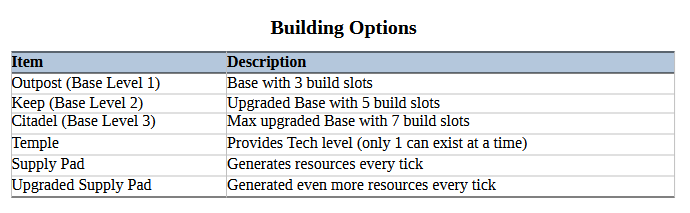
\includegraphics[width=125mm,scale=1.0]{BuildingOptionsChart.png}
			\end{center}
       		\caption{\label{fig:BuildOptions}Building and base options available to the player that affect build slot amount, economy, and tech level.}
 \end{figure}


\subsubsection{Action Requirements}
Each action and ability offers a benefit at the expense of costing resources to construct. Each ability also does not happen instantly and will take a specific amount of time for that respective ability to be performed. The table in Figure~\ref{fig:ActionsChart} contains all the relevant actions a player can do along with their respective resource and time cost. 
\newline

 \begin{figure}[!ht]
 			\begin{center}
				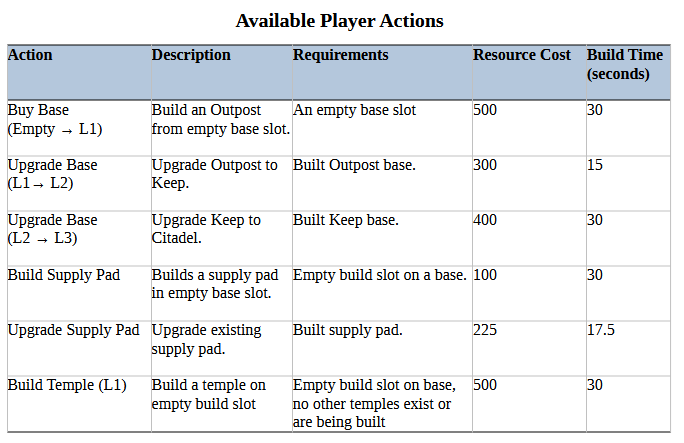
\includegraphics[width=125mm,scale=1.0]{PlayerAvailableActionsChart.png}
			\end{center}
       		\caption{\label{fig:ActionsChart}Actions along with their resource and time cost.}
 \end{figure}

 In-game, if a player attempts an action but doesn't have the requirements (e.g. does not have enough resources), no penalizing action is taken, the action is simply not completed. Additionally, in-game, once a building has been built on a build slot, there normally is an option to recycle it, which destroys the building and frees the build slot again. However, for simplicity, this project will not have the recycle option, and once a building is built it will stay in that build slot indefinitely.

\subsubsection{Starting Scenario}
With the primary actions explained, it is now important to understand how each Halo Wars game starts. When a match starts, the player begins with the following:
		\begin{itemize}
        \item A level two Base with five open build slots
        \item A Tech level of zero
        \item 800 starting resources.
  		\end{itemize}
        
The player also begins with a free "scout" unit that has basic offensive capabilities and can explore the map. There also are multiple batches of "supplies" on the map, each batch can give the player between 100-200 extra resources. The player must use unit to collect these supplies. For the sake of this project, the supplies gathered by units on the map were not calculated, since the results in-game are often inconsistent. Instead, there were some test scenarios devised to simulate resource gathering by changing the target resource threshold.
\newline

Additionally, when a player builds their Temple for the first time, they are gifted a special "Leader Unit". This unit has offensive capabilities that will be utilized in-game, but are not necessary to note in the economy simulation.

\subsubsection{Ideal/Project Scenario}
Halo wars has several "maps" that can be played, each of which offer special perks and abilities that are not otherwise available on other maps. For this project, there is one map in particular that can expedite the creation of a Scarab called "Exile". What makes Exile special is there are four "Reactors" guarded by third party hostile enemies. If the player garrisons an infantry unit they control in a reactor, their tech level increases by one as long as they hold it. It should be noted that the scout and leader units can NOT garrison the Reactors, and it needs to be done by a separate "infantry" unit.
\newline

This means if the player gets two of these reactors and builds a Temple, they will reach a tech level of three without needing to spend time and resources upgrading their Temple. This drastically speeds up the Scarab requirements completion process and over halves the resource requirements (upgrading the Temple twice cost 3000 total resources). In-game, these reactors can be cleared of hostile mobs by the players Leader Unit, as well as with help from their scout unit. In the simulation, this is assumed to happen successfully and no further calculations are required.
\newline

Additionally, to get a second base on a traditional Halo Wars map, the player has to clear out a Base Slot that is occupied by other hostile third party enemies. However, on the map Exile, there are several free Base Slots already available that can be taken with no contest. This means a second base is available to the player almost immediately, instead of normally taking two to three minutes to clear out.
\newline

Because of the advantages that the map Exile offers, the simulation assumes it will automatically have access to the Reactors and uncontested base slots. All major other assumptions are further detailed in the next section.

\subsection{Assumptions}
After understanding the major game mechanics, there are a few areas that may add either confusion or complexity. To help simplify things and create a consistent foundation for the project, the following are the major assumptions that are being accounted for.
		\begin{itemize}
        \item While a Supply Pad is being built, it does NOT produce resources.
        \item While a Supply Pad is being upgrade, it will continue to count as an un-upgraded Supply Pad until the moment the upgrade is complete. 
        \item The cost for the two extra infantry units needed for garrisoning in generators can either be added to the final resources threshold (3300), or can be ignored with the assumption that those resources would be gathered in game from supplies on the map (3000).
        \item Adding the two extra infantry units will NOT add time complexity.
        \item Assume the Reactors are cleared and populated by infantry units in time.
        \item For the the simulator, the only resources that will be added to the resource count are the resources from upgraded/non-upgraded Supply Pads, and the 800 starting resources.
        \item If going for the two Scarab stretch goal, the "Reinforcements" upgrade is required, which costs 800 additional resources (6800 total).
  		\end{itemize}


\newpage
\subsection{Game Economy}
\subsubsection{Original Equation}
Now that the player actions and project scenario has been established, a deeper look at the Halo Wars in-game economy is crucial to understating how to simulate it. 
\newline

Halo Wars uses a specialized formula that relies on how many Supply Pads and Upgraded Supply Pads a player has. Because it follows a non-linear formula, and because the variables in the formula (number and type of Supply Pads) changes over time, it makes it difficult to accurately calculate how many resources a player should have as the game progresses. The original equation for how the amount of resources are calculated was found on an online discussion form and is presented in Equation~\ref{eq:1}.

\begin{equation}
S = \frac{1.5  X}{\left(\frac{X+Y}{13}\right) + 1} + \frac{2.5 Y}{\left(\frac{X+Y}{13}\right) + 1}
\label{eq:1}
\end{equation}

\begin{itemize}
    \item $S$: Supplies per second
    \item $X$: Quantity of upgraded Supply Pads
    \item $Y$: Quantity of regular Supply Pads
\end{itemize}

\subsubsection{Modified Equation}

Initial prototype code was created and ran using this equation. However, when comparing simulation results with in game testing, it was found that this equation was slightly off, as the expected resources for even basic tests would deviate from the actual results after only a few minutes. After repeated experimentation and close analysis of expected vs actual results in a variety of situations, it was found that the following, updated equation show in Equation~\ref{eq:2} produced significantly more accurate results.
\newline

\begin{equation}
S = \frac{4.375 X}{\left(\frac{X+Y}{9}\right) + 1} + \frac{6.125 Y}{\left(\frac{X+Y}{9}\right) + 1}
\label{eq:2}
\end{equation}
\newline

The main changes being adding 1 to the X and Y coefficients and further multiplying them by another 1.75, as well as reducing the denominator from 13 to 9. Needing to modify the original equation was not unexpected, as several threads on the topic noted that the equation seemed to be from an early version of the game that had since been modified. It is likely that the actual in-game equation is different as well, as the resource value is updated every frame (60 frames a second), where as this equation calculates resources every second. 
\newline

\subsubsection{Equation Visualizations}
Several graphs were made to help visualize the relationship between upgraded or "heavy" Supply Pads,"lite" or regular Supply Pads, and how many resources they together produce a second. Figure~\ref{fig:EquationVisualization} shows the direct impact of heavy($Y$) and lite($X$) Supply Pads on the supplies per second output ($S$).
\newline

 \begin{figure}[!ht]
 			\begin{center}
				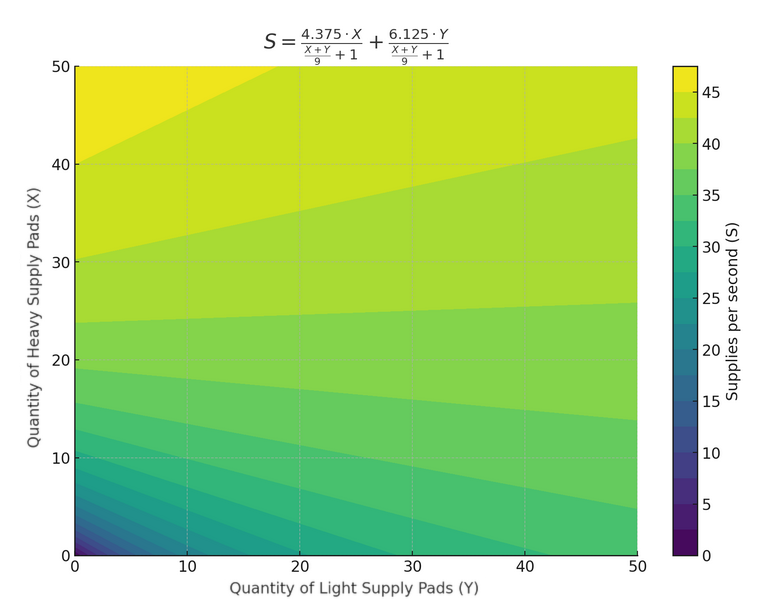
\includegraphics[width=150mm,scale=1.0]{SupplyPadGraph.png}
			\end{center}
       		\caption{\label{fig:EquationVisualization}Supply Equation Visualization.}
 \end{figure}


However, Figure~\ref{fig:EquationVisualization} only shows the direct impact that $X$ and $Y$ have on $S$, it does not take into the account the impact $X$ and $Y$ have on each other. The following is a more detailed breakdown for constructing a more truthful visualization.

\begin{itemize}
    \item Since $X$ and $Y$ relate to Supply Pads that are either built or not built, that means $X$ and $Y$ can only be integer values.
    \item Since upgraded Supply Pads can only come from un-upgraded supply Pads, $Y$ can only increase when $X$ is greater than 0.
    \item Additionally, when $Y$ increases, $X$ decreases by  the same amount
\end{itemize}


Figure~\ref{fig:XandYRelations} shows a more detailed visualization taking into account the criteria above.

\newpage

 \begin{figure}[!ht]
 			\begin{center}
				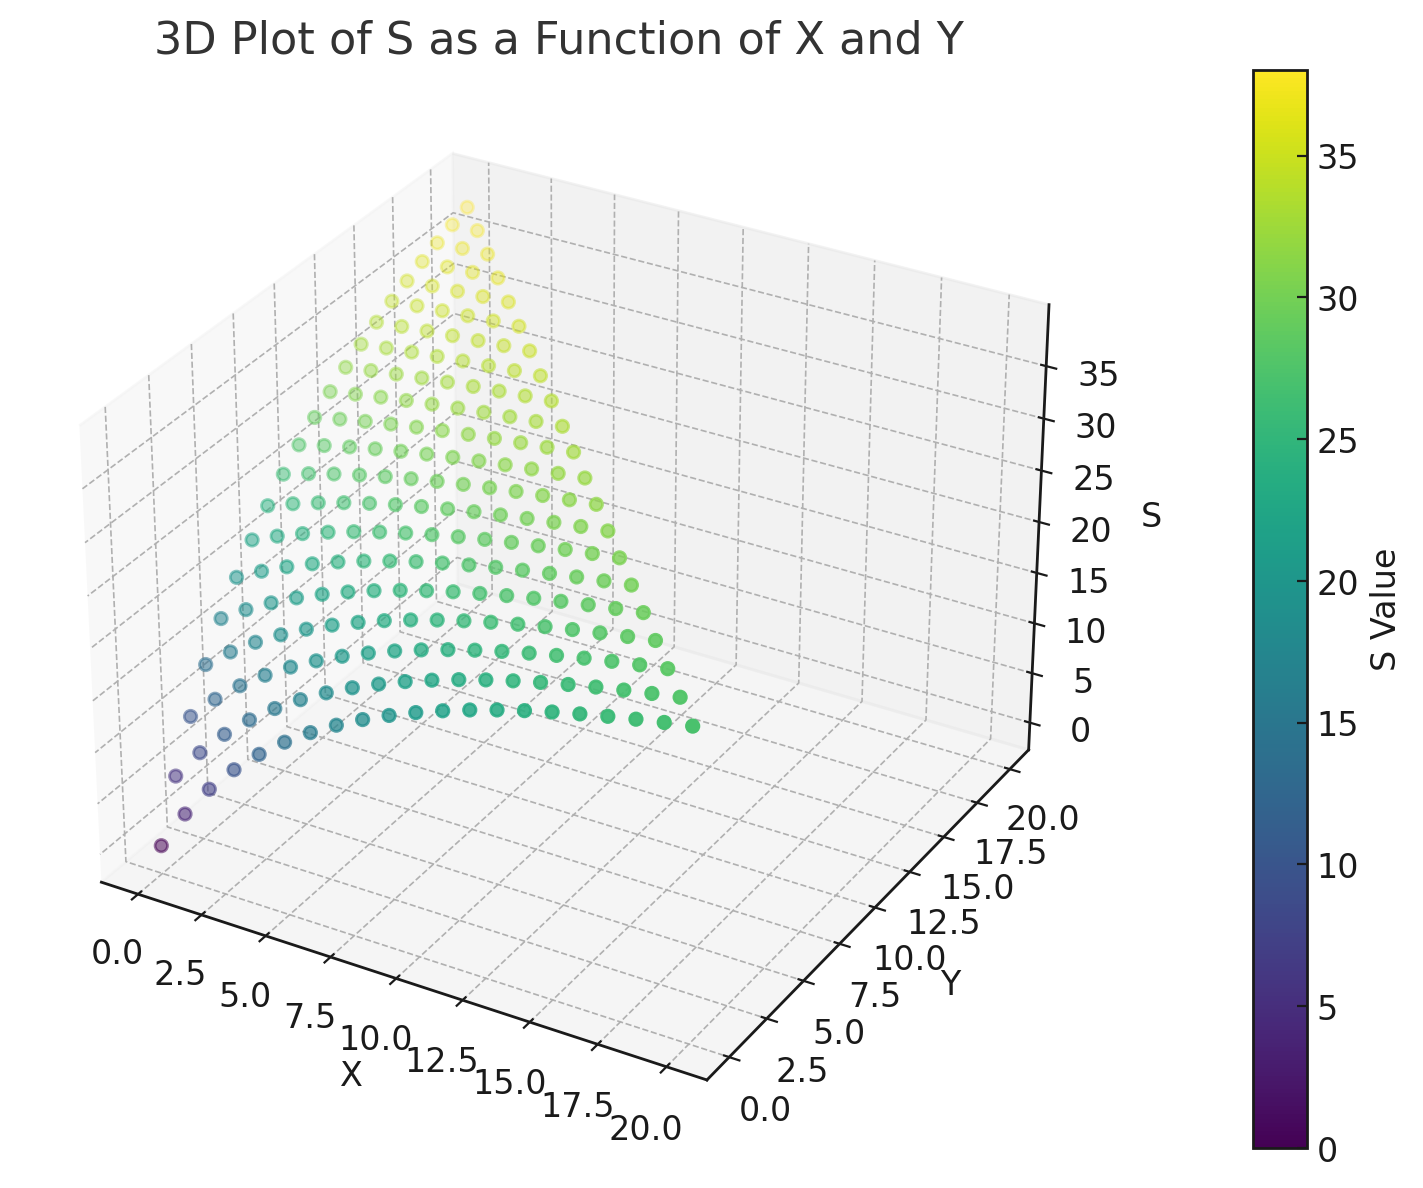
\includegraphics[width=150mm,scale=1.0]{SasfunctionofXandY.png}
			\end{center}
       		\caption{\label{fig:XandYRelations}Detailed Supply Equation Visualization.}
 \end{figure}


 Finally, Supply Pads do not just produce resources, they also cost resources to construct. The impact of $X$ and $Y$ on how many resources they cost can be visualized as well. The resource cost can be dictated as follows: 
\begin{itemize}
    \item Increasing $X$ by one cost 100 resources.
    \item Increasing $Y$ by one cost 225 resources.
\end{itemize}

 Figure~\ref{fig:XandYResources} gives a visualization of the cumulative cost when purchasing supply pads for any given combination up to twenty.

  \begin{figure}[!ht]
 			\begin{center}
				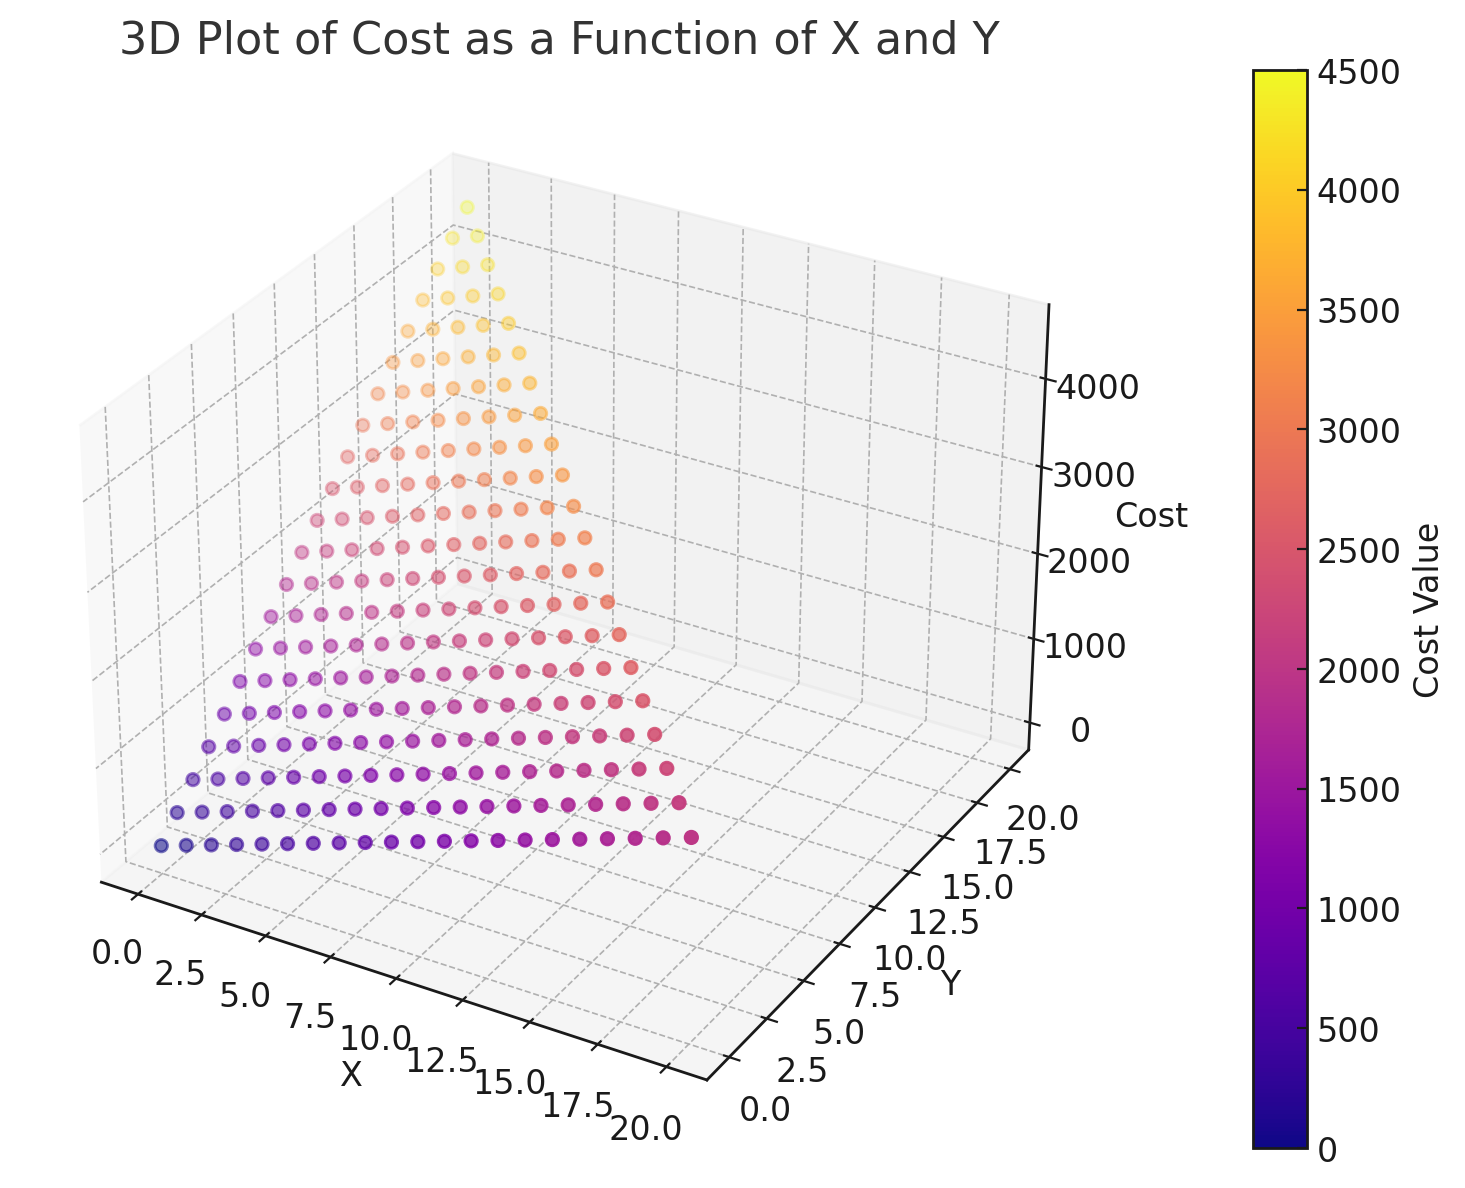
\includegraphics[width=150mm,scale=1.0]{ResourceCostForSupplyPads.png}
			\end{center}
       		\caption{\label{fig:XandYResources}Visualization of Lite and Heavy Supply Pad Costs.}
 \end{figure}

\newpage


%********************************%
%***********SECTION 3************%
%********************************%

\section{Equipment}
		\begin{itemize}
        \item  \textbf{Operating System}: Windows 10
        \item  \textbf{Development Environment}: Pycharm
        \item  \textbf{Programming Language}: Python 3.11.1
        \item  \textbf{Testing Platform}: Halo Wars Definitive Edition (Xbox One)
        
 		\end{itemize}

%********************************%
%***********SECTION 4************%
%********************************%
\newpage
\section{Methodology}

%***********************************************SUBSECTION 1************************************************%
\subsection{Introduction}
This section outlines the methodology used to develop the Halo Wars economy simulator and build order optimizer. The approach consisted of designing a Python-based simulator, developing a way to test different build orders, and combining these components to identify the fastest Scarab build strategy.
\newline

\subsection{Overall Design}
The simulator aimed to mimic the in-game mechanics of Halo Wars. Those mechanics, described in the previous sections, primarily involve resource generation calculations, building construction timing, and upgrade timing. To achieve this, Python was used to create this simulator, utilizing object oriented programming and software design principals.  
\newline

Several prototypes were explored, but the final result involved having the simulator take in a "build order"—a list of sequential actions to execute—and calculate the time required to reach a specific resource threshold. To identify the fastest build order, a secondary program was created to generate random build orders for the simulator to evaluate. The idea behind random build orders was that if enough random orders were generated, the fastest build order, or at least certain trends, could be found.  
\newline

The project was divided into two main components:
\begin{itemize}
    \item \textbf{Simulator program:} Kept track of build times and the resource collection rates, outputting the time required to reach a given resource threshold in in-game seconds.
    \item \textbf{Build order generator:} Generated randomized build orders to feed into the simulator for evaluation. Certain redundancy and verification checks were utilized to provide only valid build orders to the simulator.
\end{itemize}

Once developed, the two components were integrated using a simulator wrapper and supporting classes to streamline execution and analysis.
\newline

\subsection{Python Simulation Components Design}
The simulator was designed with a modular architecture consisting of three primary components:
\begin{itemize}
    \item \textbf{Base class:} Managed base operations, including construction, upgrades, and build timers.
    \item \textbf{BuildSlot class:} Represented individual build slots for constructing and upgrading buildings.
    \item \textbf{ResourceManager class:} Oversaw resource and technology level updates to ensure consistency.
\end{itemize}

\subsubsection{Base Class}
\begin{figure}[!ht]
    \begin{center}
        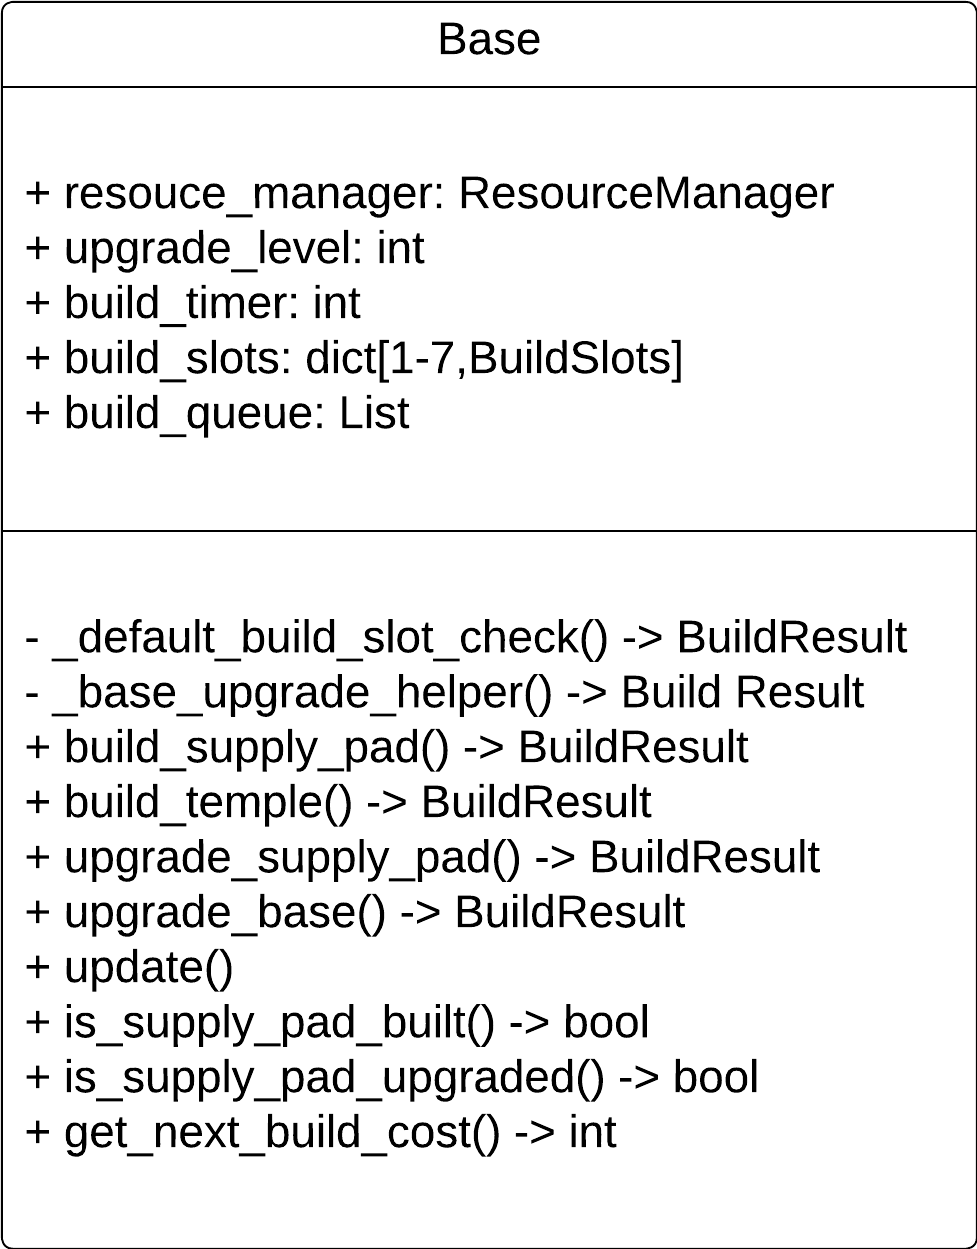
\includegraphics[width=60mm,scale=1.0]{HaloWarsDiagramBase.png}
    \end{center}
    \caption{\label{fig:BaseClass}Base Class}
\end{figure}

The \textbf{Base} class modeled individual bases in the game. Each base has up to seven build slots and operates independently, with its own build timers and slot assignments. This independence ensures accurate simulation of multi-base gameplay, where actions on one base do not interfere with others.  
\newline

Key methods include:
\begin{itemize}
    \item \texttt{build\_supply\_pad()} and \texttt{build\_Temple()}: For constructing Supply Pads and Temples.
    \item \texttt{upgrade\_base()} and \texttt{upgrade\_supply\_pad()}: For upgrading bases and Supply Pads.
    \item \texttt{update()}: Called every in-game second to manage build timers and update associated build slots.
\end{itemize}

Additionally, the class implemented a \textbf{BuildResult} enumeration to provide detailed feedback on action outcomes (e.g., \texttt{NOT\_ENOUGH\_RESOURCES}, \texttt{APPROVED}). A \textbf{BaseState} enumeration tracked the base's status (e.g., \texttt{IDLE}, \texttt{UPGRADING}).  
\newline


\subsubsection{BuildSlot Class}
\begin{figure}[!ht]
    \begin{center}
        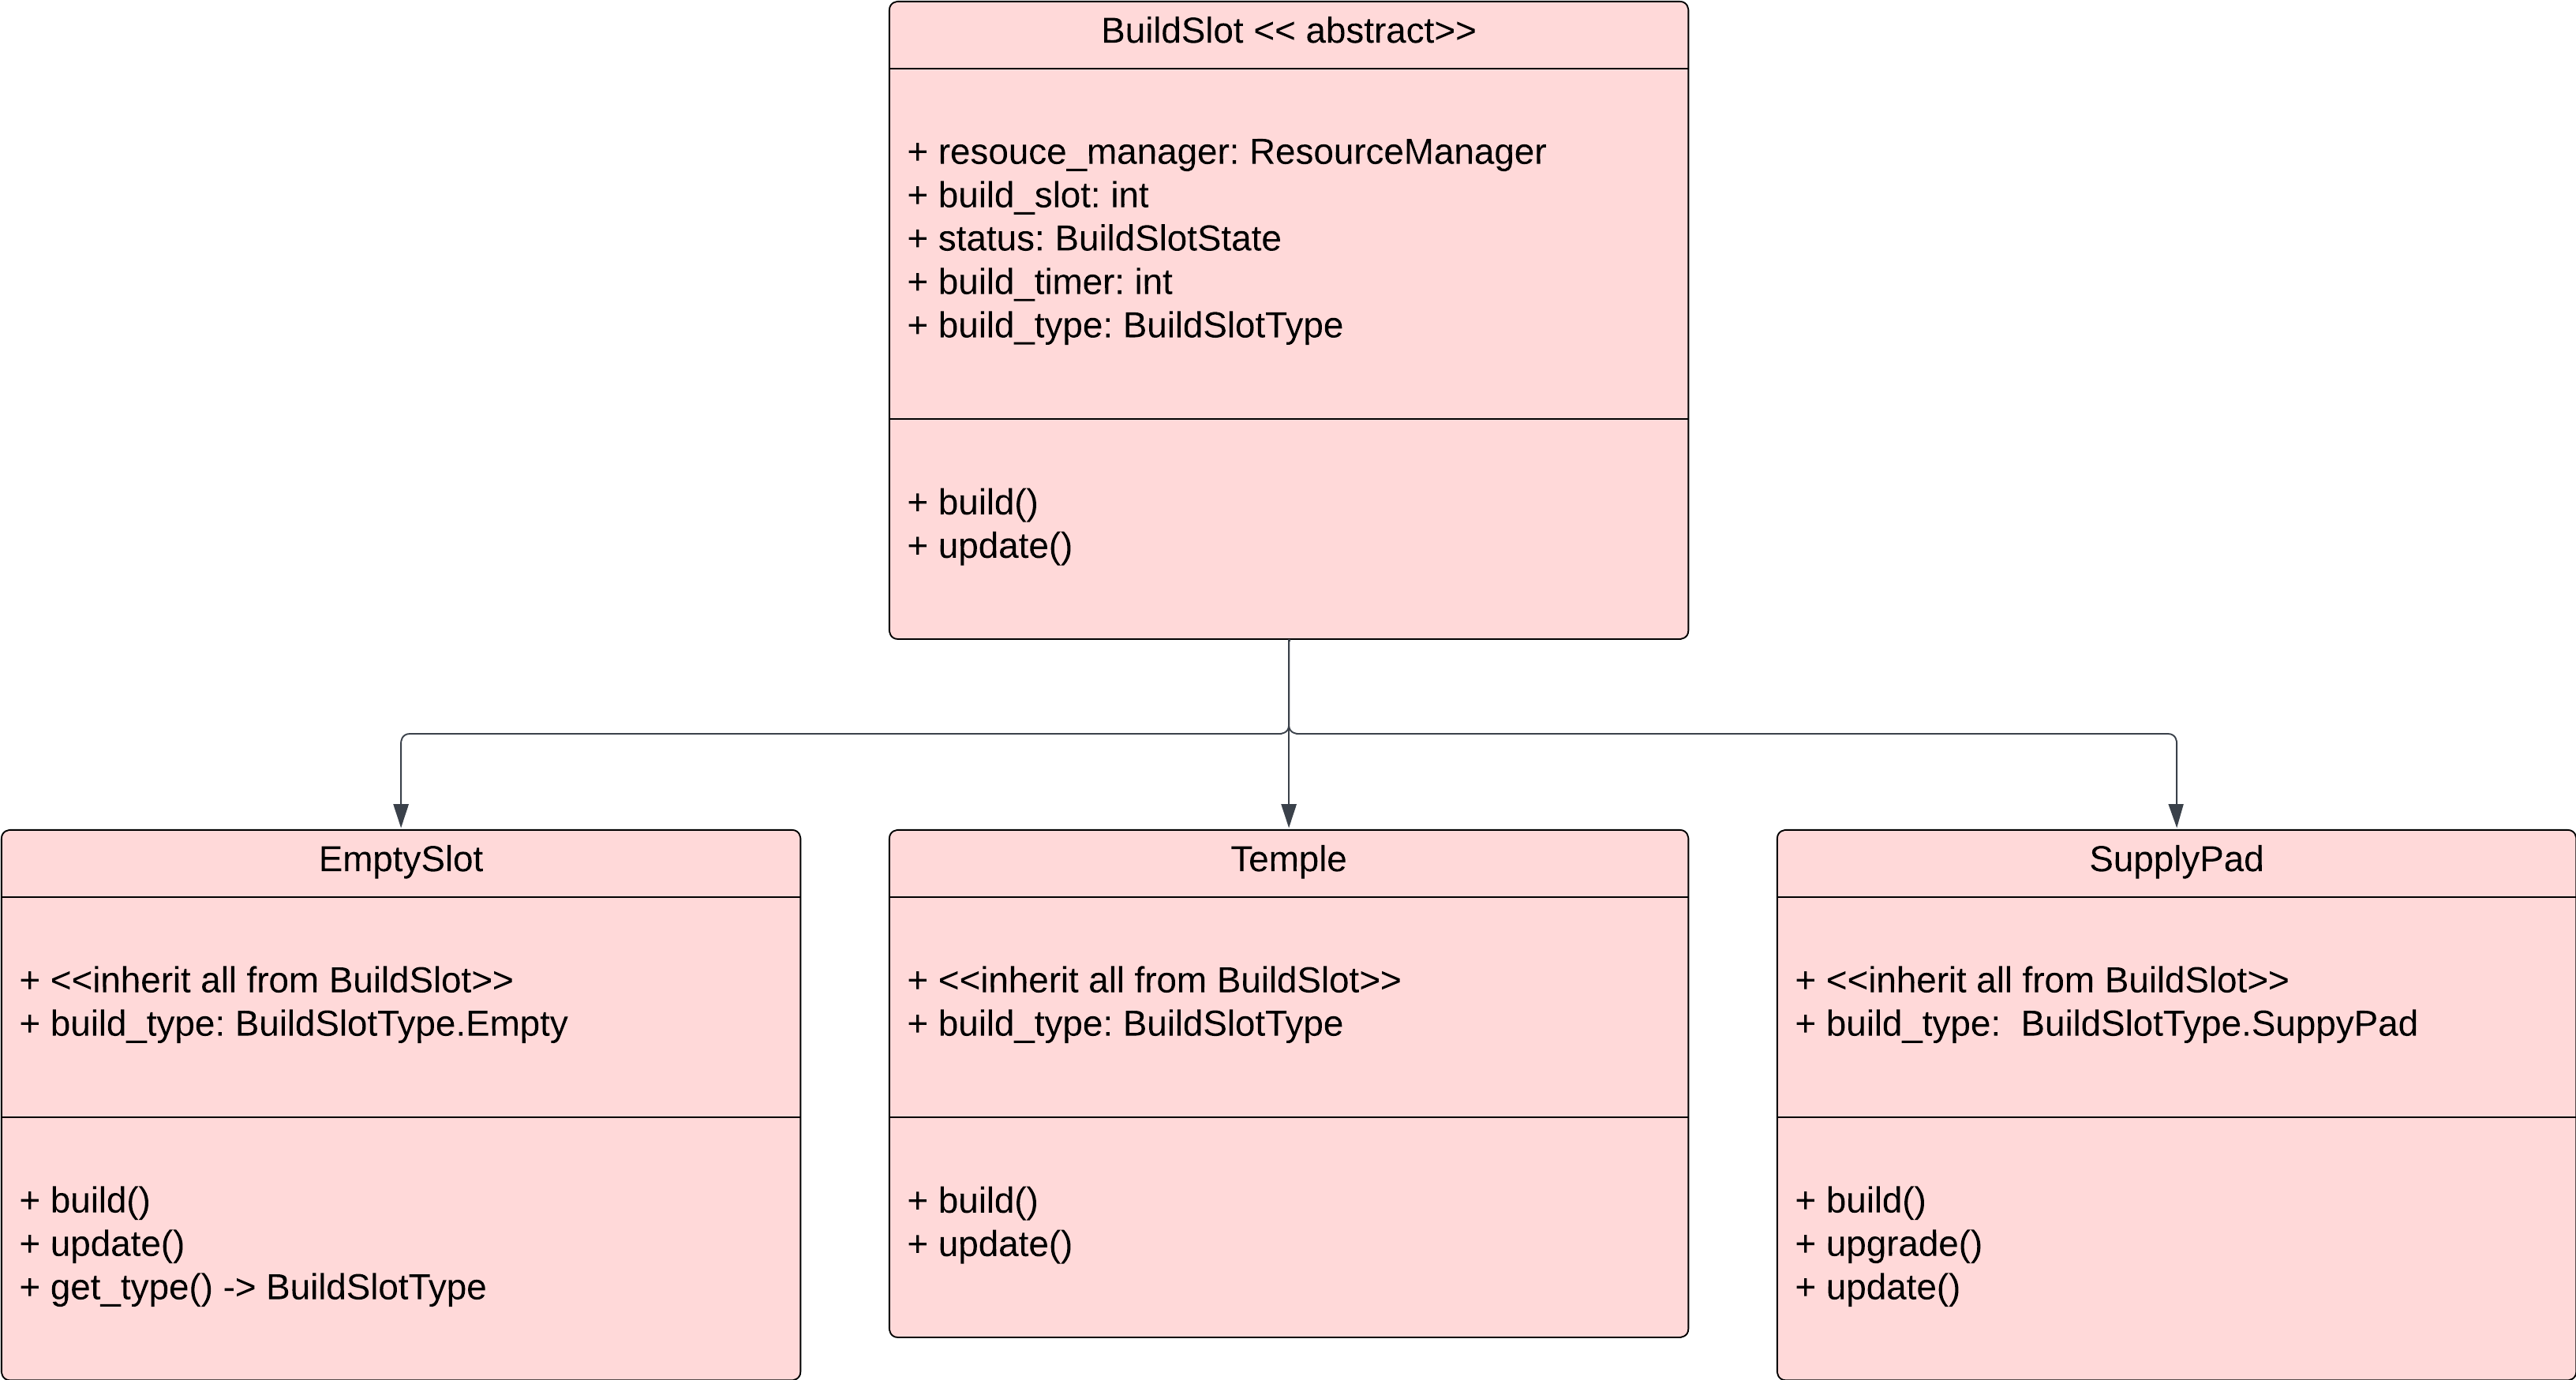
\includegraphics[width=150mm,scale=1.0]{HaloWarsDiagramBuildSlots.png}
    \end{center}
    \caption{\label{fig:BuildSlotClass}BuildSlot Class}
\end{figure}

The \textbf{BuildSlot} class served as an abstract foundation for all building types. Subclasses included:
\begin{itemize}
    \item \textbf{EmptySlot:} Default state of unused build slots, facilitating checks for available slots.
    \item \textbf{SupplyPad:} Handled Supply Pad construction, upgrades, and interactions with the ResourceManager.
    \item \textbf{Temple:} Managed Temple construction and tech level updates.
\end{itemize}

By centralizing resource management within build slot classes, the design minimized the risk of errors, such as duplicate or untracked buildings. Constants for build costs and times were stored in a separate configuration file for easy modification.

\subsubsection{ResourceManager Class}
\begin{figure}[!ht]
    \begin{center}
        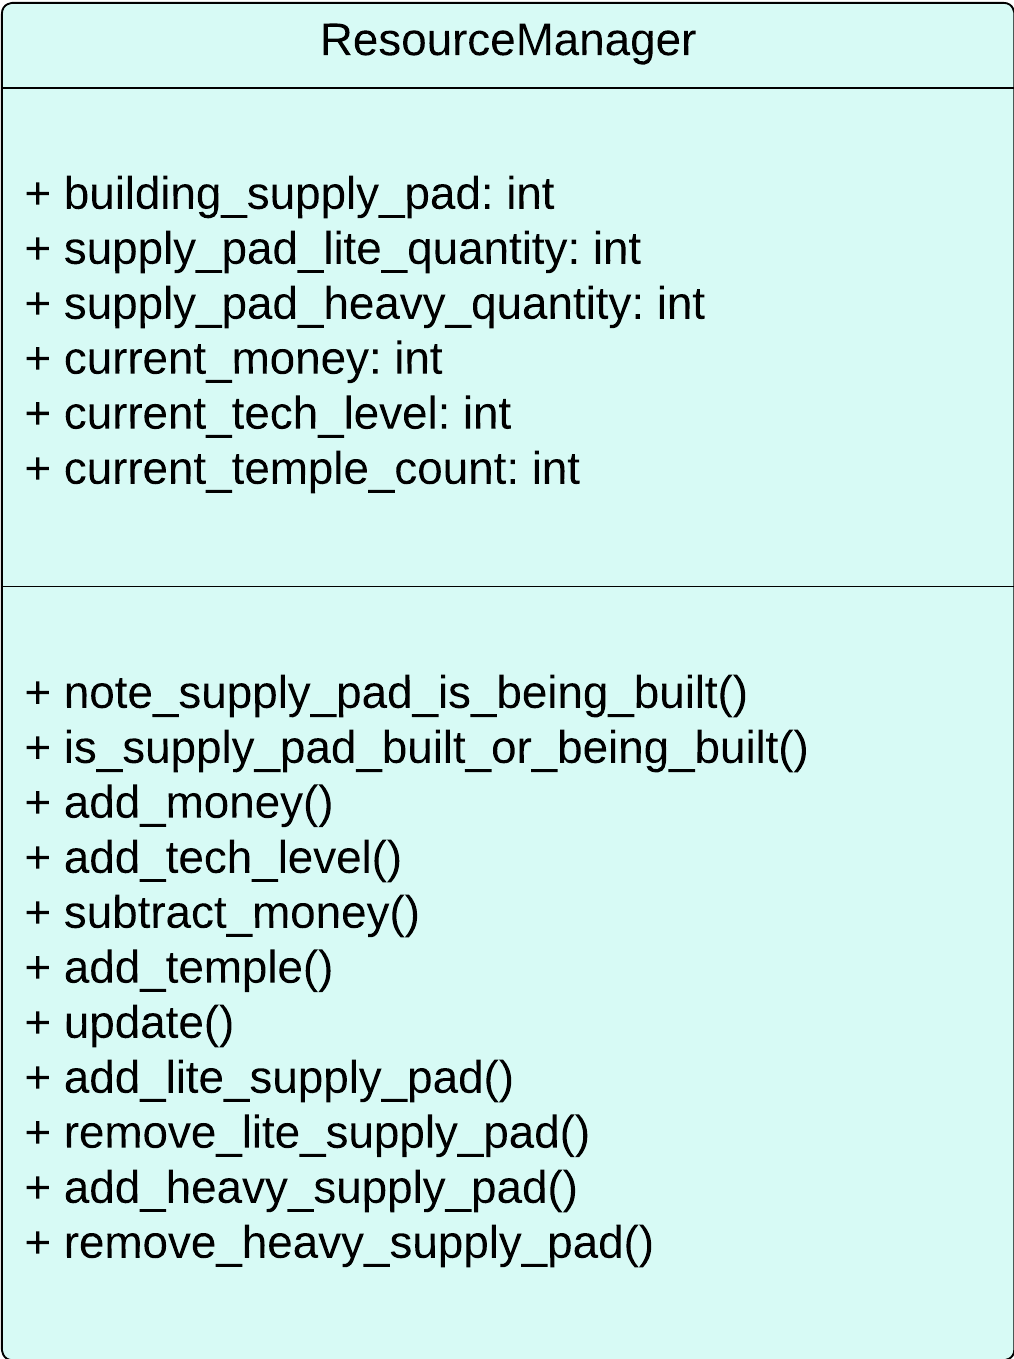
\includegraphics[width=60mm,scale=1.0]{HaloWarsDiagramResourceManager.png}
    \end{center}
    \caption{\label{fig:ResourceManagerClass}ResourceManager Class}
\end{figure}

The \textbf{ResourceManager} class centralized resource and technology level tracking, ensuring consistency across the simulation.  

Key variables included:
\begin{itemize}
    \item \texttt{current\_money}: Tracked the player’s resource balance.
    \item \texttt{current\_tech\_level}: Tracked the player’s technology level.
    \item \texttt{supply\_pad\_lite\_quantity} and \texttt{supply\_pad\_heavy\_quantity}: Count regular and upgraded Supply Pads.
    \item \texttt{building\_supply\_pad}: Tracked whether a Supply Pad was under construction.
\end{itemize}

Core methods:
\begin{itemize}
    \item \texttt{add\_money()} and \texttt{subtract\_money()}: Managed resource transactions.
    \item \texttt{add\_tech\_level()}: Updated the tech level, allowing for future flexibility beyond the current use case.
    \item \texttt{update()}: Calculated resource generation each in-game second using the Supply Pad formula.
\end{itemize}

\subsubsection{Combining the Simulator Classes}

With all core components now developed, a working program existed that could accurately predict the Halo Wars economy when the Objects were manually controlled. Figure~\ref{fig:SimulatorUML} shows the relationship between these classes and how they operated together.
\newline


\begin{figure}[!ht]
    \begin{center}
        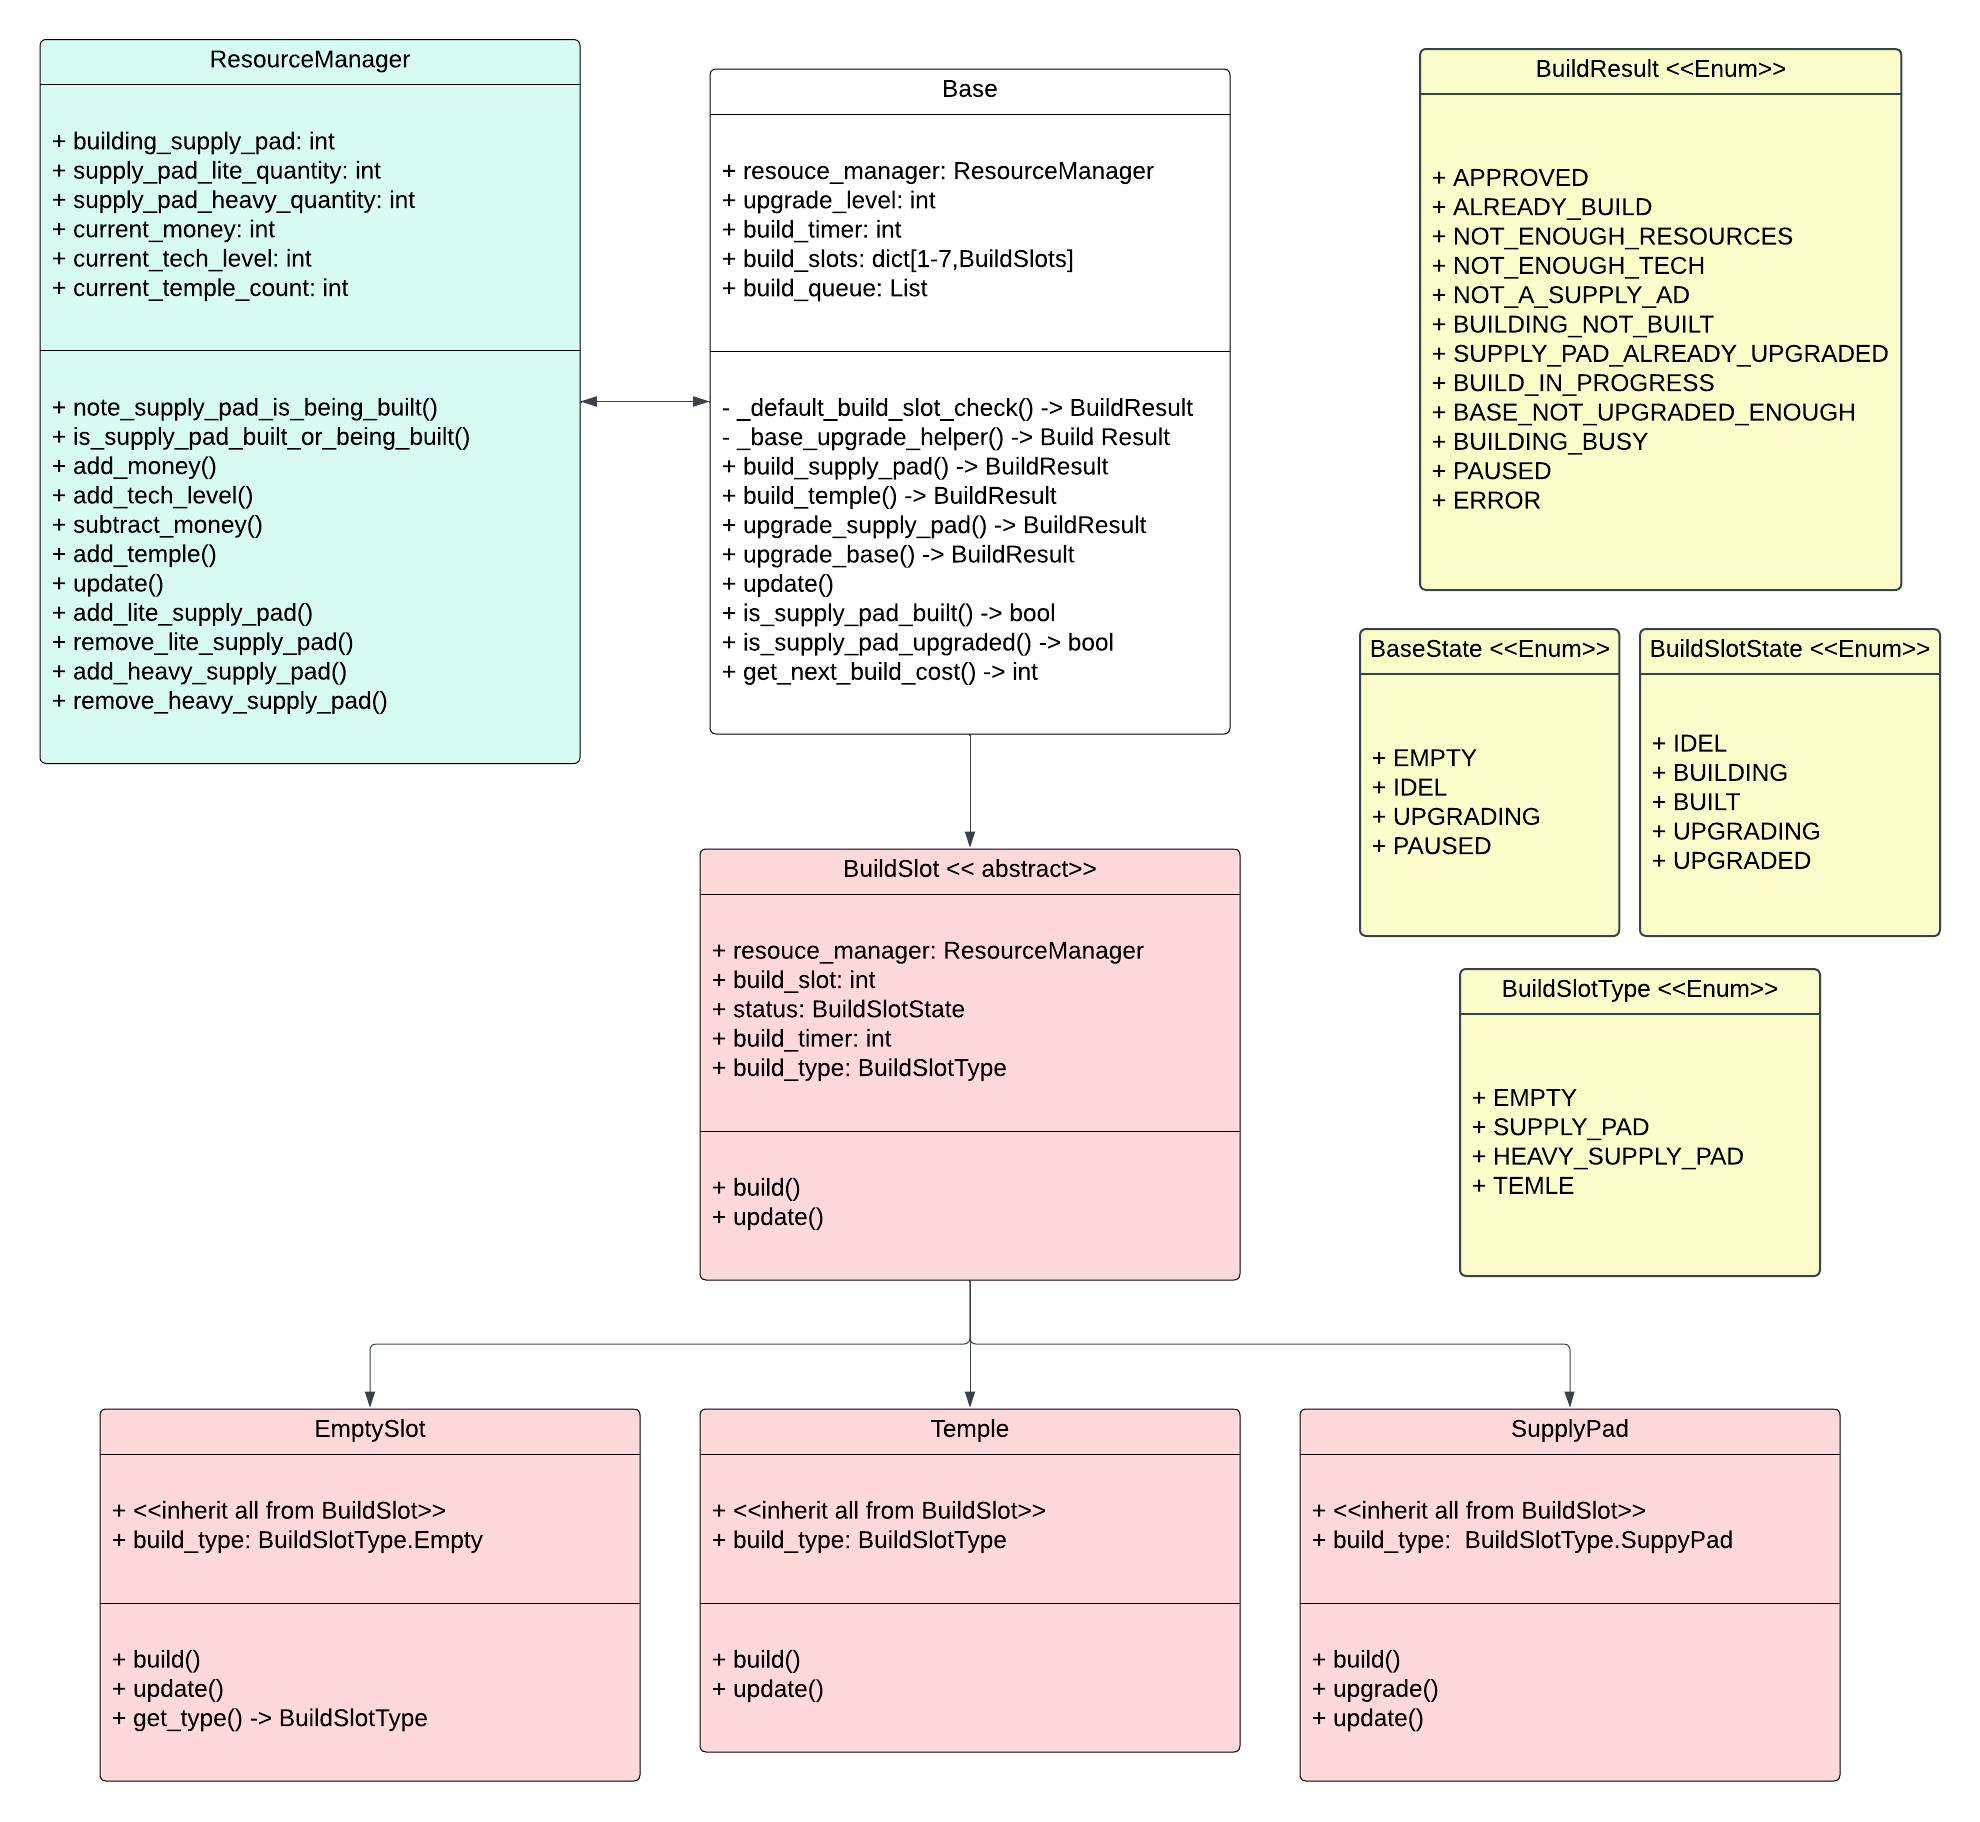
\includegraphics[width=150mm,scale=1.0]{HaloWarsDiagram.png}
    \end{center}
    \caption{\label{fig:SimulatorUML}Basic Halo Wars Simulator UML Diagram}
\end{figure}


However, another class was needed that could take in the build order list and turn it into actionable commands the simulator could execute on. For that, the \textbf{RuntimeBuildingBlocks} class was created to coordinate their interactions. This class included:
\begin{itemize}
    \item \texttt{run\_simulator()}: Executed build orders and calculated the time required to reach a resource threshold.
    \item \texttt{build\_verifier()}: Validated and executed individual build actions.
\end{itemize}

The \texttt{run\_simulator()} method output the time taken to reach a resource threshold in integer format. The output time and the respective build order details are used in the eventual wrapper class to add the results to the final results list, and eventual CSV file. Figure~\ref{fig:RuntimeBlocks} illustrates the relationships between the components, specifically how the \textbf{RuntimeBuildingBlocks} takes in the build order list, Base references, and resource trigger limit, and can feed it properly to the Simulator.
\newline

Note, the \texttt{run\_simulator()} method was designed to attempt to run every build order. If there was an order to perform a build or upgrade, but there was not enough resources, the simulator was programmed to wait until enough resources are generated before executing and proceeding.

\begin{figure}[!ht]
    \begin{center}
        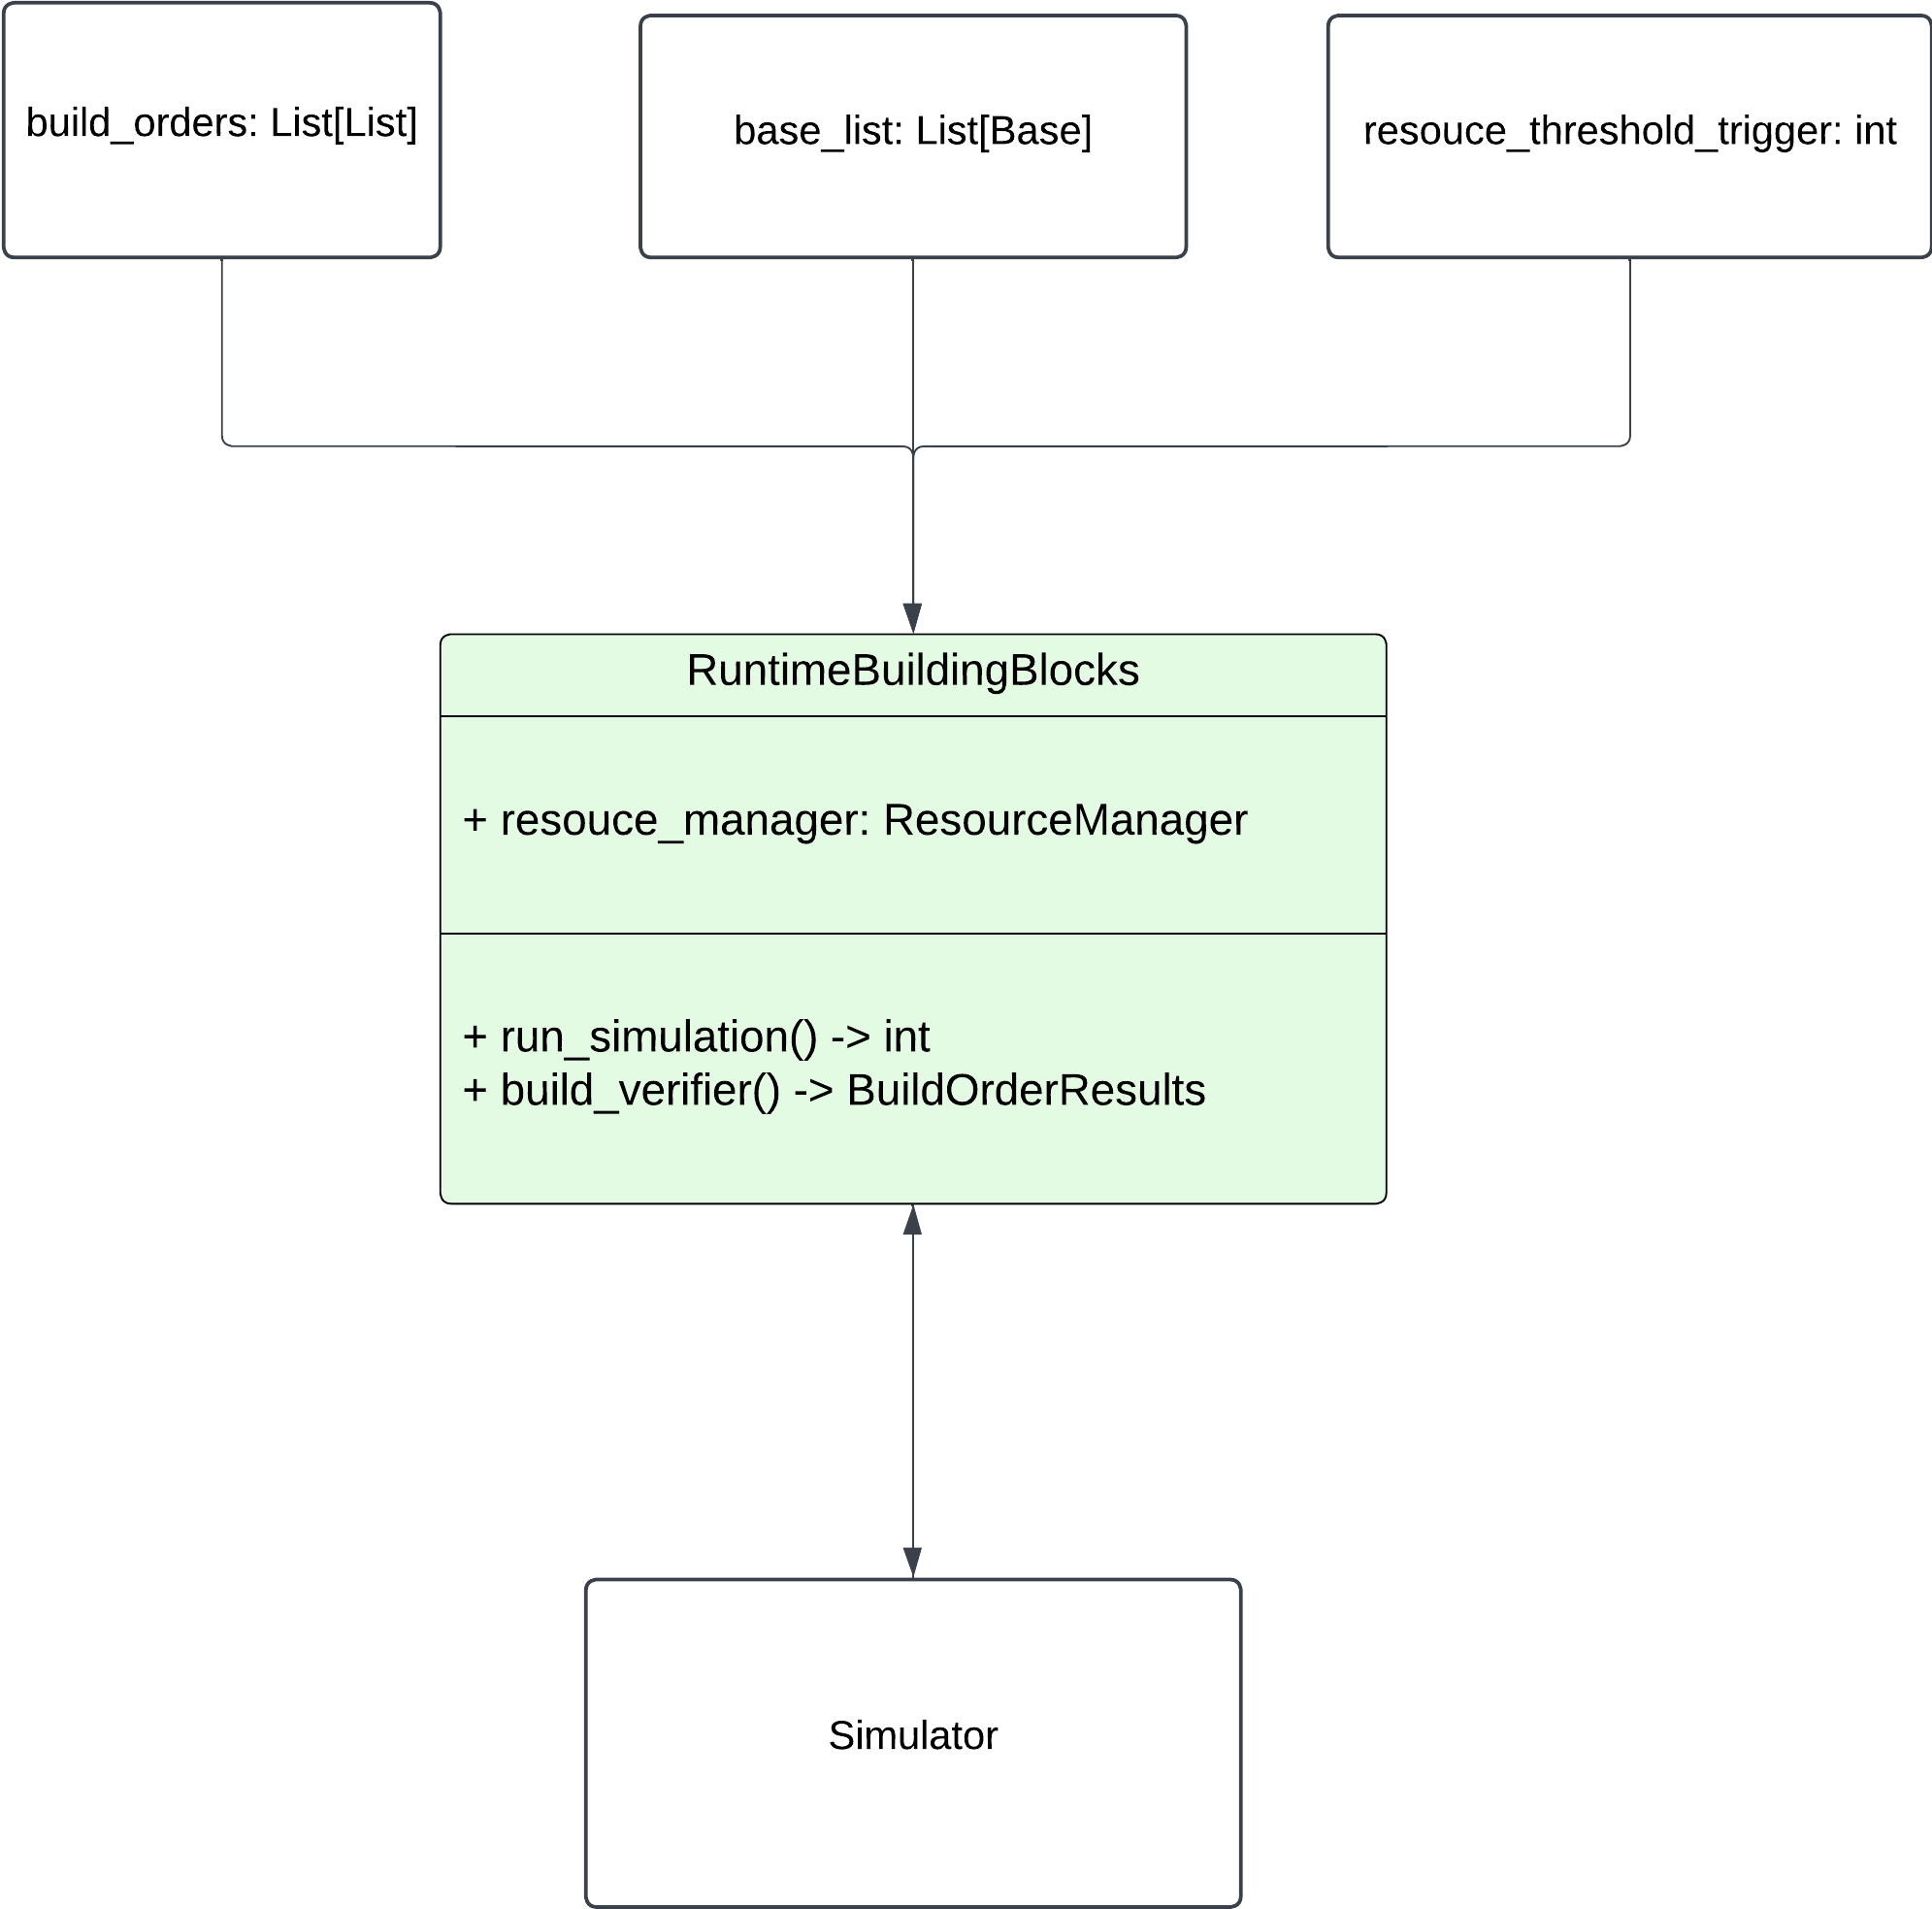
\includegraphics[width=110mm,scale=1.0]{HaloWarsDiagramRuntimeBuildingBlocks.png}
    \end{center}
    \caption{\label{fig:RuntimeBlocks}RuntimeBuildingBlocks Relationship}
\end{figure}




\newpage
\subsection{Python Build Order Program Design}

\subsubsection{Build Order List Structure}
The concept of "Build Orders" was central to the program's functionality. After experimentation, the final structure consisted of creating a list of Build Orders that could be read by the program. The orders in the list would give information for performing specific actions that the program would try to execute. Each order consisted of three key components:
\newpage
\begin{itemize}
    \item \textbf{Order Enumeration:} Specifies the action to perform, including:
        \begin{itemize}
            \item \texttt{BUILD\_SUPPLY\_PAD}
            \item \texttt{BUILD\_TEMPLE}
            \item \texttt{UPGRADE\_BASE}
            \item \texttt{UPGRADE\_SUPPLY\_PAD}
        \end{itemize}
    \item \textbf{Base Number:} An integer reference to the base where the order is executed.
    \item \textbf{BaseSlotNumber:} Indicates the build slot for building-related orders. For base-related actions (e.g., upgrades), this field was not used.
\end{itemize}

These values were stored in individual lists, which were then combined into a larger \texttt{BuildOrderList} representing the full sequence of actions. This design allowed the simulator’s \texttt{RuntimeBuildingBlocks} class to iterate through the build order, execute each step, and calculate the time required to reach a specific resource threshold. Figure~\ref{fig:BuildOrderExample} illustrates an example build order generated in Python.

\begin{figure}[!ht]
    \begin{center}
        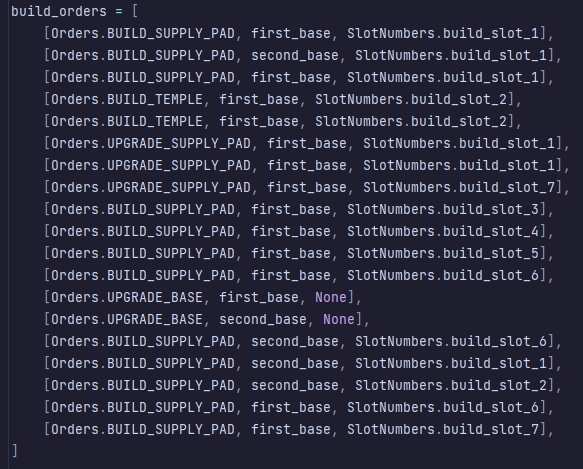
\includegraphics[width=125mm,scale=1.0]{BuildOrderListExample.png}
    \end{center}
    \caption{\label{fig:BuildOrderExample}Example Build Order List}
\end{figure}

\newpage
\subsubsection{Generating Build Orders}
The original, most pressing question of this project was how to find the optimal build order. Initially, statistical methods were explored to determine every possible combination of build orders. However, that proved to be too difficult, so the idea of generating random build orders was born. 
\newline

A program was developed to generate these random build orders and specific safety checks would ensure they were non-repeating and valid. The main caveat with this method was that sufficient iteration coverage was needed to increase the likelihood of finding the optimal solutions.
\newline

The core methodology was implemented in the \texttt{GenerateOrdersBuildingBlocks} class and followed these steps:
\begin{itemize}
    \item A \textbf{maximum build order length} was defined (default: 28).
    \item A random number determined the length of the build order that was to be generated (how many total orders).
    \item A list of currently built bases was tracked, and a random base was selected.
    \item A random action was chosen based on predefined probabilities:
        \begin{itemize}
            \item Actions such as \texttt{BUILD\_SUPPLY\_PAD} or \texttt{UPGRADE\_SUPPLY\_PAD} had higher probabilities due to their frequent use.
            \item Unique actions like building a \texttt{Temple} were assigned lower probabilities.
        \end{itemize}
    \item These probabilities were stored as adjustable parameters to allow easy tuning during testing and development.
\end{itemize}

This randomization approach efficiently generated diverse build orders. Figure~\ref{fig:OrderGeneratorClass} provides an overview of the \texttt{GenerateOrdersBuildingBlocks} class.

\begin{figure}[!ht]
    \begin{center}
        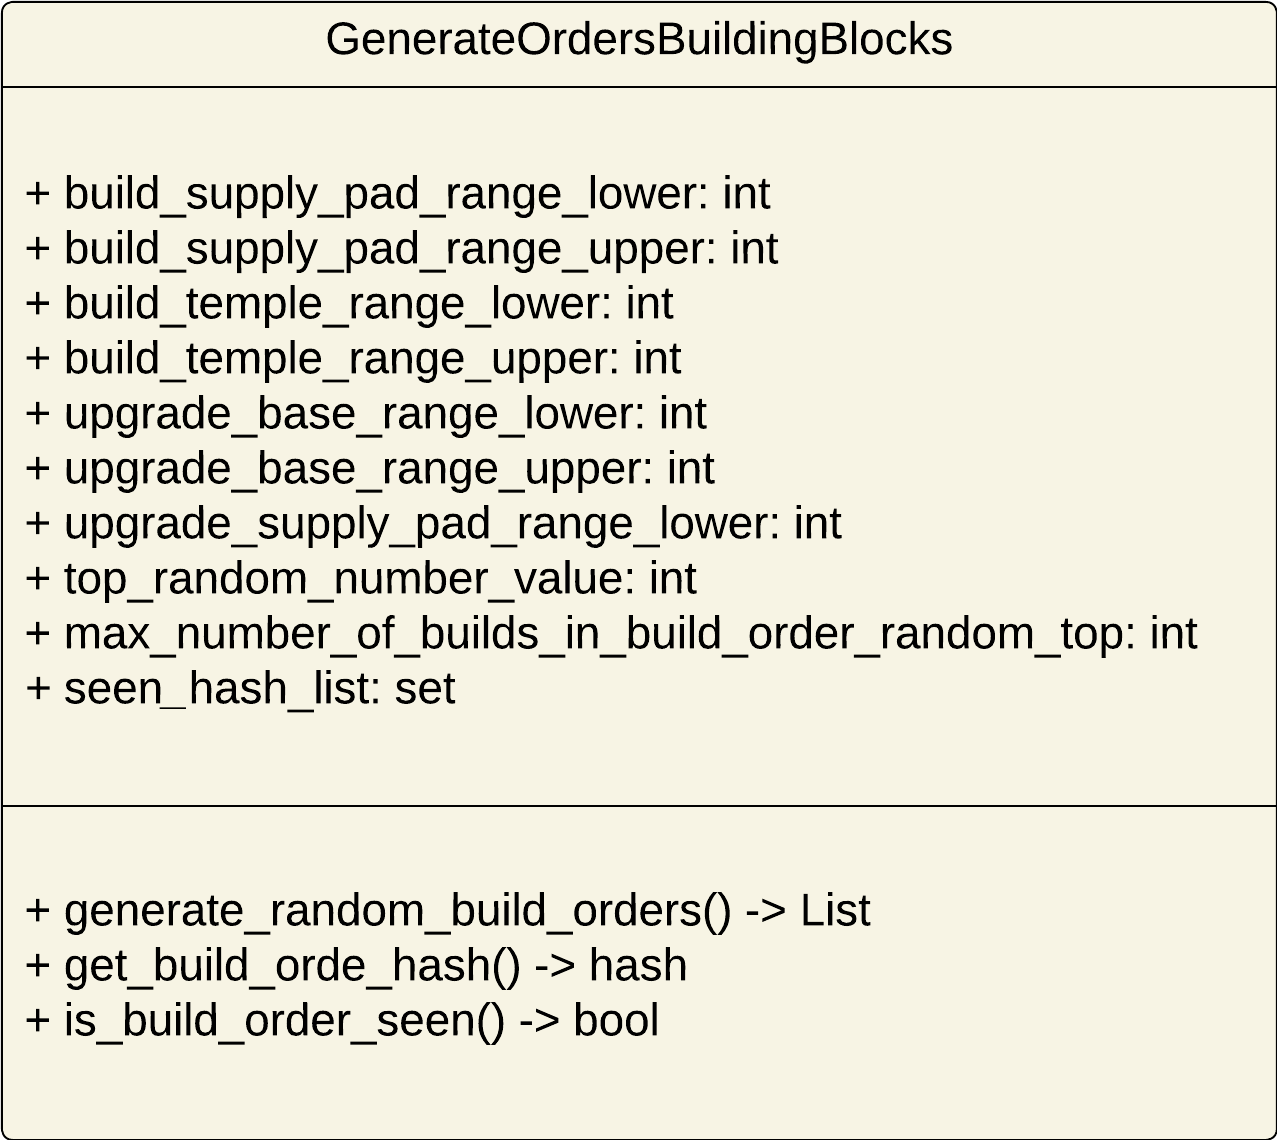
\includegraphics[width=75mm,scale=1.0]{HaloWarsDiagramGenerateOrdersBuildingBlocks.png}
    \end{center}
    \caption{\label{fig:OrderGeneratorClass}GenerateOrdersBuildingBlocks Class}
\end{figure}

\subsubsection{Build Order Safety Mechanisms}
To ensure valid and efficient build orders, several safeguards were implemented:
\begin{itemize}
    \item The \texttt{BaseBuildCounters} class tracked key metrics such as the number of bases, their upgrade levels, available slots, and built structures.
    \item Build orders were validated during generation to prevent invalid actions (e.g., exceeding the number of available slots for Supply Pads).
    \item Helper variables, such as \texttt{build\_index}, were used to sequentially assign actions to appropriate slots, minimizing randomness in slot allocation.
    \item A flag was made that could be toggled to ensure a Temple was in the build order (when first testing, none of the fastest build orders contained temples, which was invalid).
\end{itemize}

For example, the \texttt{build\_index} ensured that Supply Pads are assigned to available slots in order, while a separate \texttt{temple\_index} tracked the Temple slot to avoid conflicts with Supply Pad upgrades. Figure~\ref{fig:BaseBuildCountersClass} illustrates the \texttt{BaseBuildCounters} class.

\begin{figure}[!ht]
    \begin{center}
        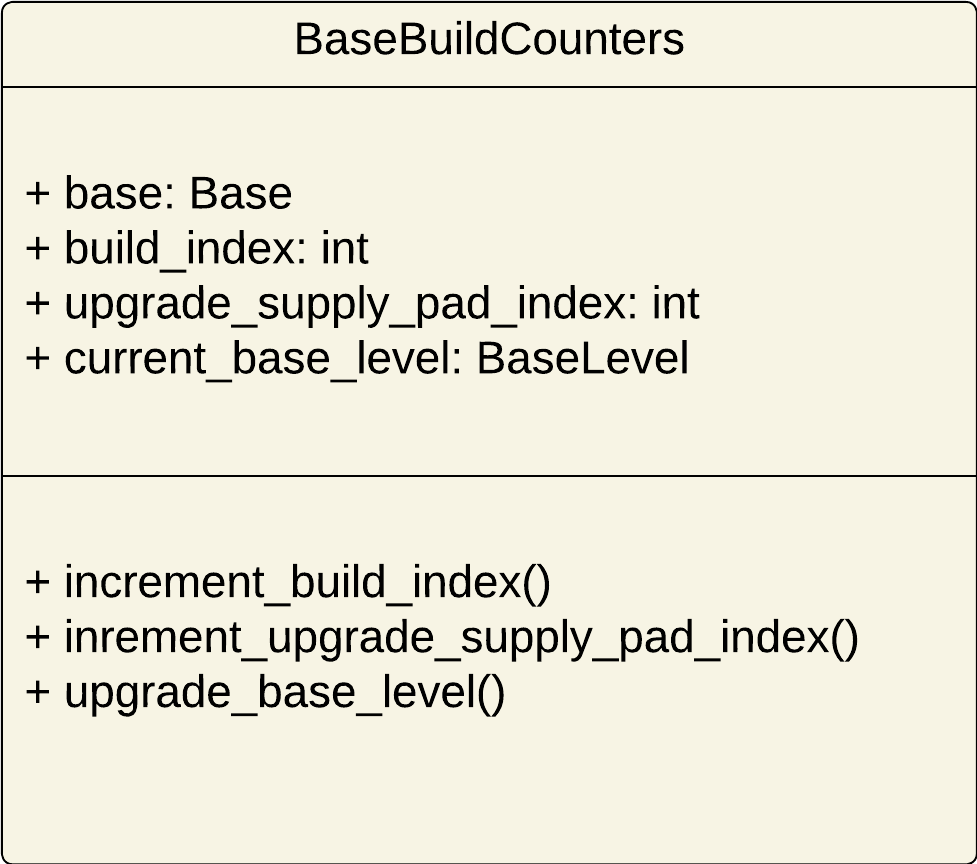
\includegraphics[width=75mm,scale=1.0]{HaloWarsDiagramBaseBuildCounters.png}
    \end{center}
    \caption{\label{fig:BaseBuildCountersClass}BaseBuildCounters Class}
\end{figure}

\newpage
\subsubsection{Checking for Redundancies}
To avoid duplicate build orders, a hash-based system was implemented:
\begin{itemize}
    \item Each generated build order was hashed and checked against a set called \texttt{seen\_hash\_list}.
    \item If the hash was already present, the build order was discarded; otherwise, it was added to the output list.
\end{itemize}

This approach reduced computational overhead compared to iterative comparisons. Since this method stored the hashes in a set, it had a lookup complexity of \(O(1)\) instead of \(O(n)\) if the program were to attempted to find duplicates by looking through the build order list directly. This also highlights the use of efficient data structures such as hash sets, aligning with the project’s focus on leveraging Python's strengths. Figure~\ref{fig:HashBasedValidation} shows the overall build generation and validation workflow.

\begin{figure}[!ht]
    \begin{center}
        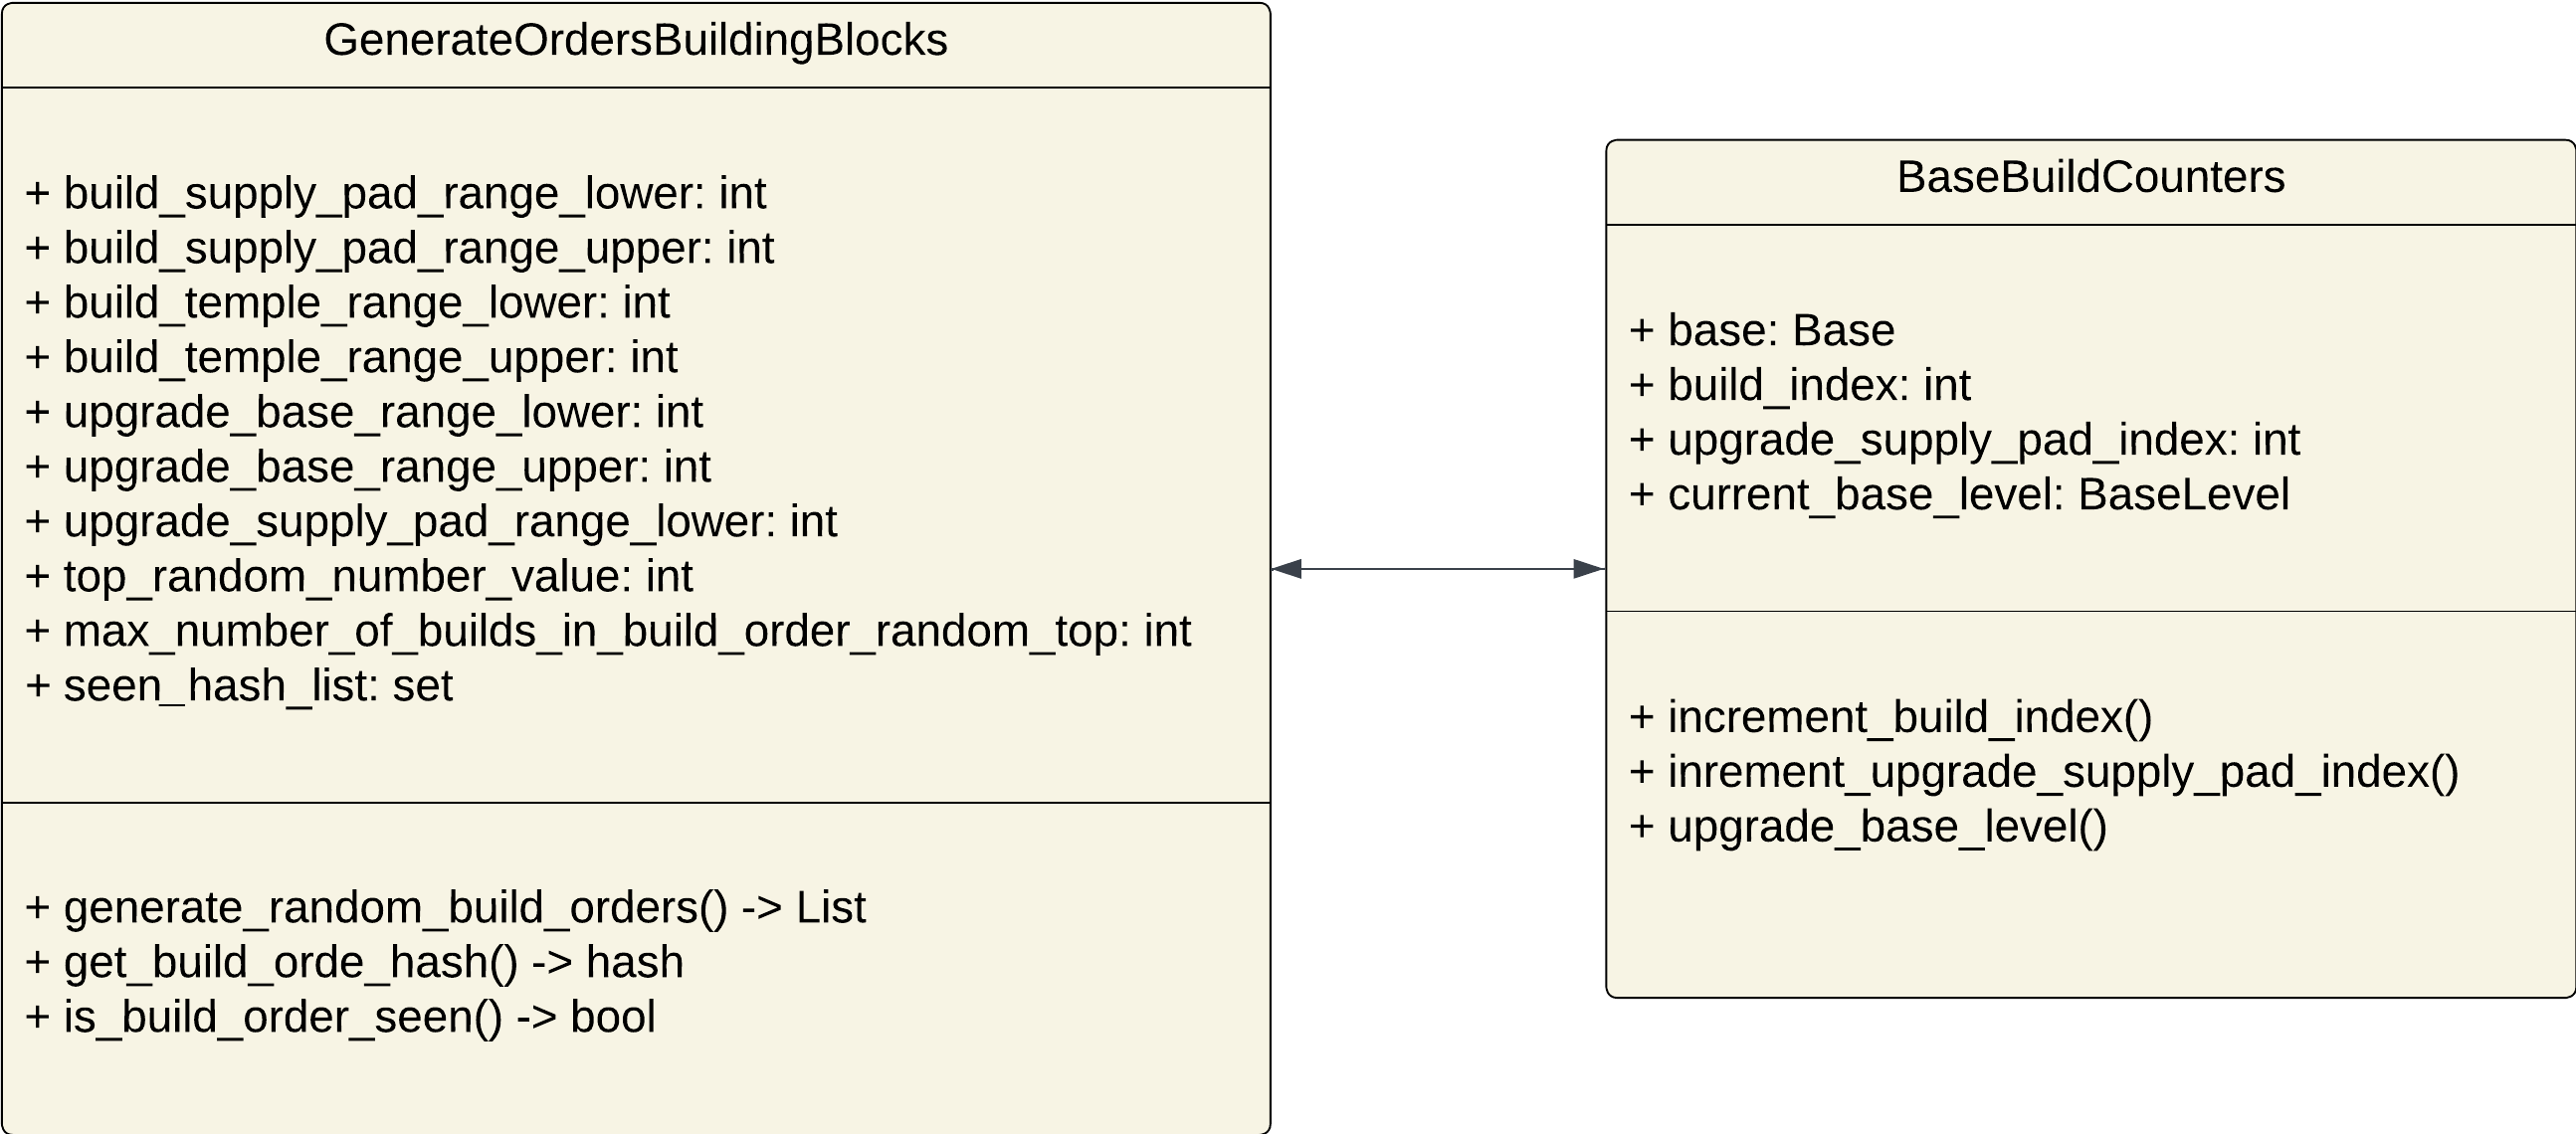
\includegraphics[width=150mm,scale=1.0]{HaloWarsDiagramOrderGenerationOverview.png}
    \end{center}
    \caption{\label{fig:HashBasedValidation}Build Generation Overview}
\end{figure}


\subsection{Merging the Two Products}

With the primary simulator classes, build order generation mechanisms, and validation systems complete, the project was ready to integrate all components into a cohesive workflow. Figure~\ref{fig:HighLevelOverview} illustrates the high-level relationships between these systems.

\begin{figure}[!ht]
    \begin{center}
        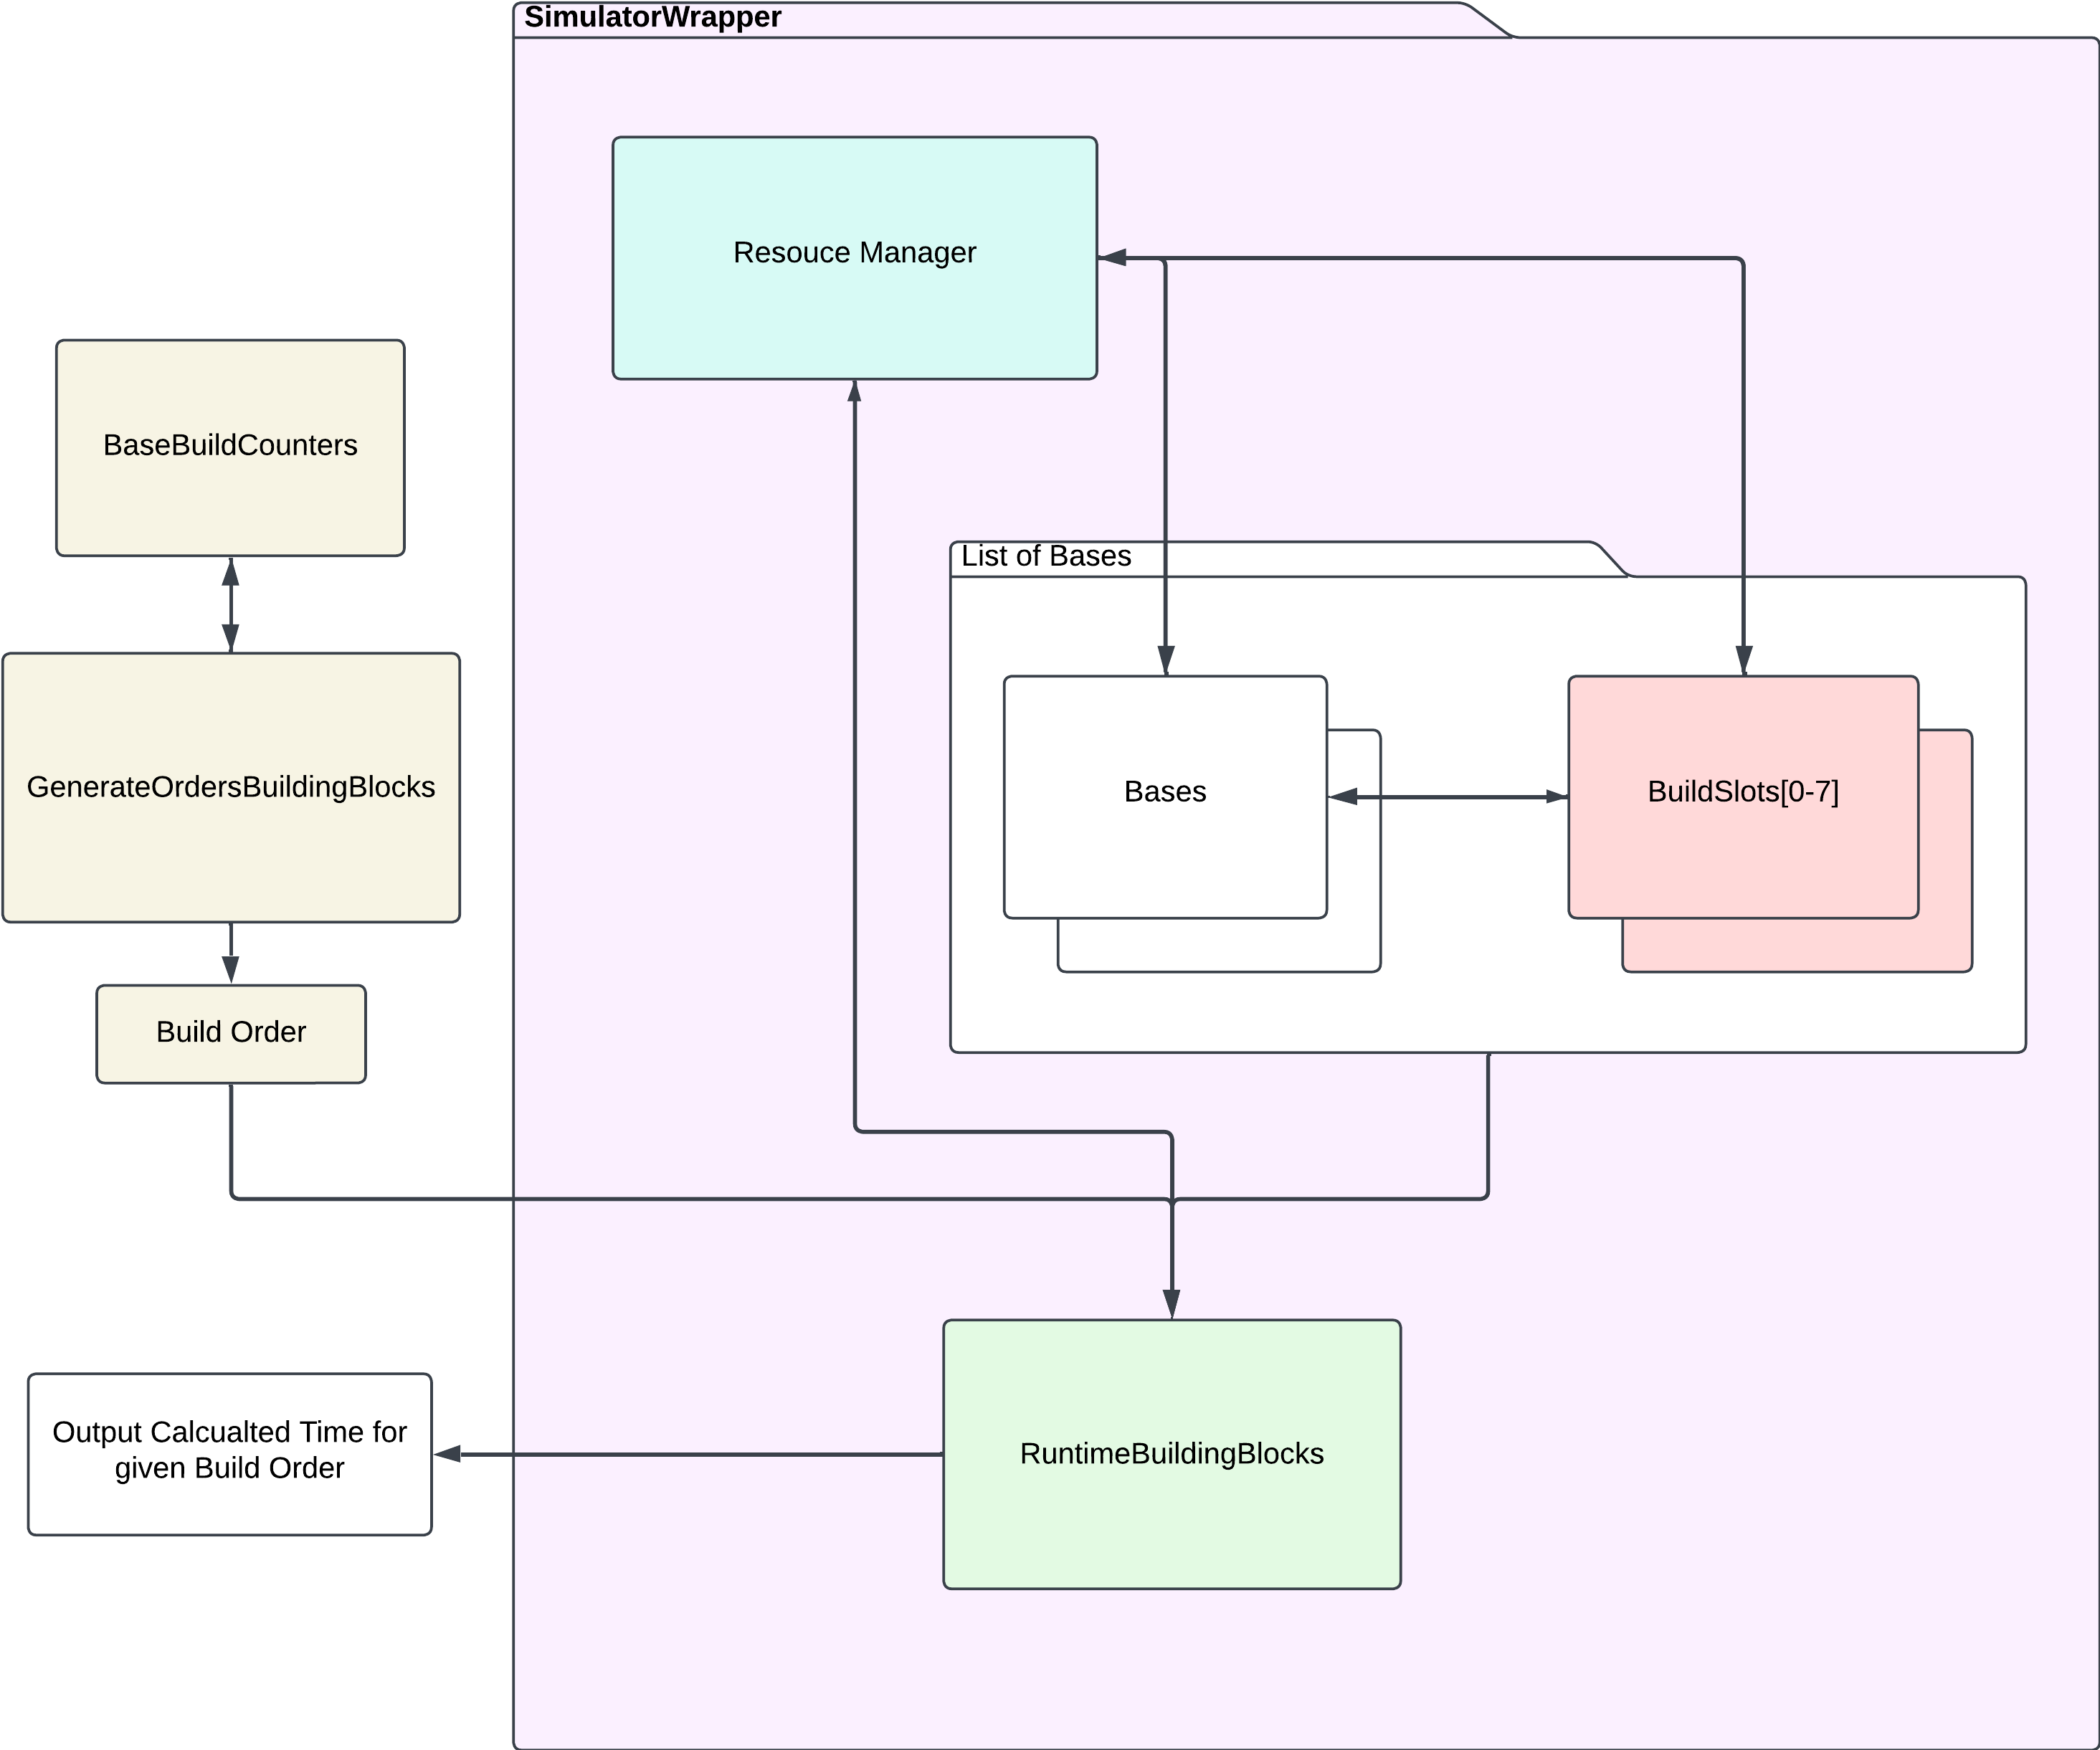
\includegraphics[width=150mm,scale=1.0]{HaloWarsDiagramHighLevelOverview.png}
    \end{center}
    \caption{\label{fig:HighLevelOverview}High-Level Overview of Class Relationships}
\end{figure}

The integration process followed these steps:
\begin{itemize}
    \item \textbf{Build Order Generation:} The \texttt{GenerateOrdersBuildingBlocks} class would create a randomized, non-repeating build order for testing.
    \item \textbf{Resource Manager and Base Initialization:} The \texttt{ResourceManager} was then instantiated and linked to all \texttt{Base} and \texttt{BuildSlot} objects. These components were further referenced by the \texttt{RuntimeBuildingBlocks} class, enabling it to manage build orders effectively.
    \item \textbf{Simulation Wrapper:} The \texttt{SimulationWrapper} class consolidated all simulation-related objects, simplifying their initialization and providing a single interface for executing simulations.
    \item \textbf{Main Program Execution:} The final integration was handled by the \texttt{run\_build\_combinations.py} program, which served as the primary driver for the system. Its workflow included:
        \begin{itemize}
            \item Initializing the \texttt{SimulationWrapper} and \texttt{GenerateOrdersBuildingBlocks} classes.
            \item Managing constant values, such as maximum simulation time, starting resources, resource value triggers, and the number of bases, through easily adjustable parameters at the top of the file.
            \item Iterating through the main simulation loop:
                \begin{itemize}
                    \item A new build order gets generated. If it is unique, the simulator calculates the time required to reach a predefined resource threshold. If not, the build order is skipped.
                    \item The calculated time and corresponding build order are added to a results list.
                    \item Repeat for as many times as defined by the \texttt{NUMBER\_OF\_SIMULATION\_LOOPS} constant.
                    \item Once the simulation loop completes, results export all results to a CSV file.
                \end{itemize}
        \end{itemize}
    \item \textbf{Fail-Safe Mechanisms:} The \texttt{run\_simulation} method included a maximum simulation time threshold. If the simulation exceeded this threshold, the iteration was terminated, and the system proceeded to the next build order.
\end{itemize}

This complete integration formed the foundation for an automated system capable of generating, validating, and simulating build orders at scale. Results were saved to a CSV file for further analysis, providing both calculated build times and the corresponding build orders.
\newline

In addition to the primary simulation program, a secondary utility program, \texttt{halo\_wars\_supply\_pad\_simulator.py}, was created, which allows users to input manually created build lists, such as the one shown in Figure~\ref{fig:BuildOrderExample}. This utility was primarily used for testing and debugging purposes.
\newline

Users could adjust the \texttt{NUMBER\_OF\_SIMULATION\_LOOPS} constant to control the number of iterations and rerun the program as needed. Future updates may include support for command-line arguments, enabling batch testing with varying parameters.
\newline


\newpage
\section{Results}
\subsection{Overview}

Testing focused on three adjustable parameters: the resource threshold, the number of bases, and the number of build order iterations. The experimental design and parameters are detailed below.

\subsubsection{Resource Threshold}
    \begin{itemize}
    \item \textbf{3000 Resources}: The threshold to acquiring a Scarab with the assumption that supplies on map cover the two infantry units.
    \item \textbf{3300 Resources}: Similar to 3000-resource threshold but without the assumption the infantry cost is covered.
    \item \textbf{6800 Resources}: The threshold to construct two Scarabs. An additional 800 resources beyond the 6000 required for two scarabs is included to purchase the "Reinforcements" upgrade.
    \end{itemize}

\subsubsection{Base Limits}
The number of bases ranged from one to two, as typically only one additional base is accessible to the player early in gameplay. Some testing was done with three bases, but it typically produced results only using two bases, ignoring the third.
\newline

\subsubsection{Build Order Iterations}
The number of iterations was the greatest unknown, it was unsure how many iterations were needed, so this value was adjusted to balance execution time and result reliability. Testing started out small at 100 iterations and incremented by factors of 10, reaching 100,000. These iteration runs would take between 5-10 minutes to execute, so the iterations were increased again to 200,000. One 500,000 iteration run was attempted, however, due to its execution time of about 45 minutes, higher iterations counts were deemed impractical for subsequent tests.
\newline


\subsubsection{Build Order Terminology}
The following keywords are used to describe build orders in the results tables:
    \begin{itemize}
    \item \textbf{U\_BASE}: Upgrade the base, if there is no base in the base slot, build the base.
    \item \textbf{SUPPLY}: Build a Supply Pad.
    \item \textbf{U\_SPLY}: Upgrade an existing Supply Pad.
    \item \textbf{TEMPLE}: Build a Temple.
    \item \textbf{1 or 2}: Numbers following keywords indicate the base to which the action corresponds.
    \end{itemize}
    

\newpage
\subsection{3000 Resources Threshold}
The following figures shows the results for the values gathered from the runs with one and two bases, set to a 3000 resource threshold, and variable iterations. 

 \begin{figure}[!ht]
 			\begin{center}
				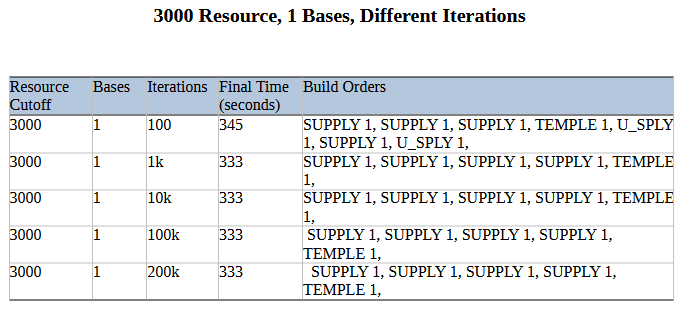
\includegraphics[width=150mm,scale=1.0]{3000r1b.png}
			\end{center}
       		\caption{\label{fig:Lowpass}One Base 3000 Resource Threshold}
 \end{figure}


 \begin{figure}[!ht]
 			\begin{center}
				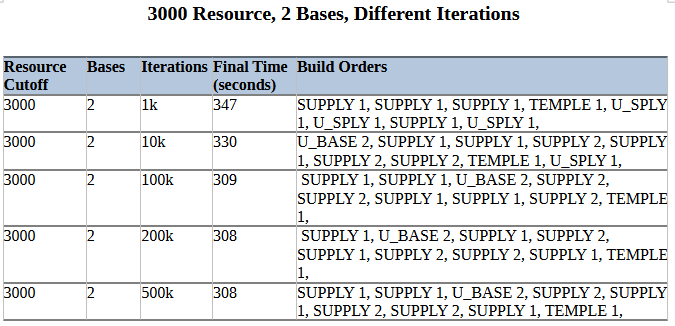
\includegraphics[width=150mm,scale=1.0]{3000r2b.png}
			\end{center}
       		\caption{\label{fig:Lowpass}Two Base 3000 Resource Threshold}
 \end{figure}


\newpage
\subsection{3300 Resources Threshold}

The following figures shows the results for the values gathered from the runs with one and two bases, set to a 3300 resource threshold, and variable iterations.

 \begin{figure}[!ht]
 			\begin{center}
				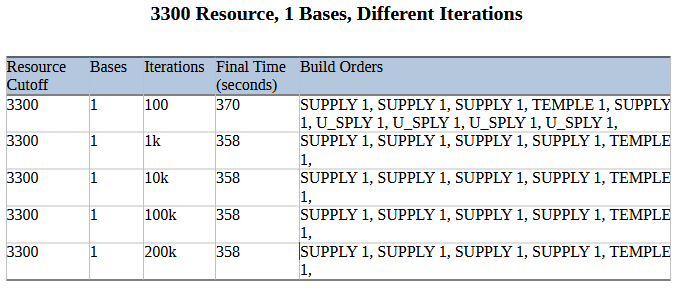
\includegraphics[width=150mm,scale=1.0]{3300r1b.png}
			\end{center}
       		\caption{\label{fig:Lowpass}One Base 3300 Resource Threshold}
 \end{figure}


 \begin{figure}[!ht]
 			\begin{center}
				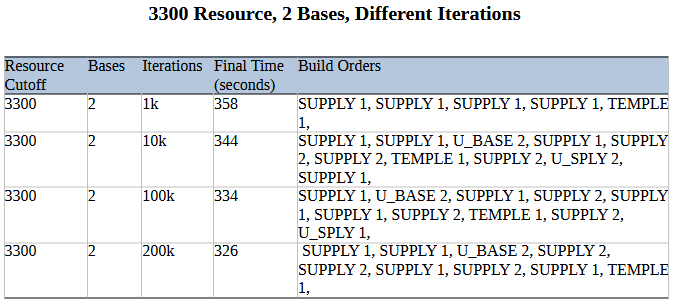
\includegraphics[width=150mm,scale=1.0]{3300r2b.png}
			\end{center}
       		\caption{\label{fig:Lowpass}Two Base 3300 Resource Threshold}
 \end{figure}

\newpage
\subsection{6800 Resources Threshold}

The following figures shows the results for the values gathered from the runs with one and two bases, set to a 6800 resource threshold, and variable iterations.

 \begin{figure}[!ht]
 			\begin{center}
				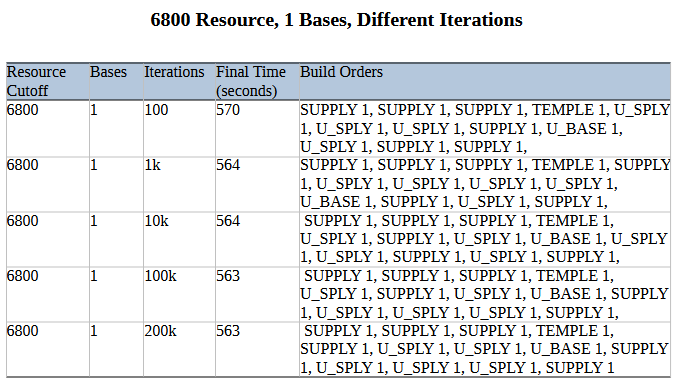
\includegraphics[width=150mm,scale=1.0]{6800r1b.png}
			\end{center}
       		\caption{\label{fig:Lowpass}One Base 6800 Resource Threshold}
 \end{figure}


 \begin{figure}[!ht]
 			\begin{center}
				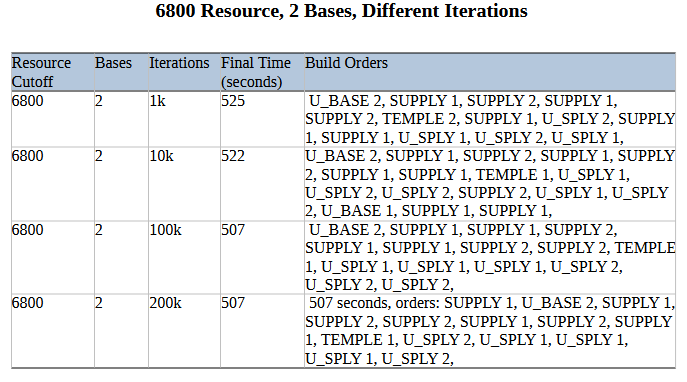
\includegraphics[width=150mm,scale=1.0]{6800r2b.png}
			\end{center}
       		\caption{\label{fig:Lowpass}Two Base 6800 Resource Threshold}
 \end{figure}


\newpage
\subsection{Final Results}

The following sections present the final results of the simulations and in-game testing for constructing one and two Scarabs, highlighting both build orders and resource timings.

\subsubsection{Simulated Final Results: One Scarab}

The fastest simulated result for reaching 3000 resources and constructing a Scarab with two bases was achieved in \textbf{308 seconds}. The corresponding build order was as follows:  
\begin{itemize}
    \item Build two Supply Pads on Base 1.
    \item Immediately construct a second base.
    \item Sequentially build additional Supply Pads:
    \begin{itemize}
        \item Supply Pad on Base 2.
        \item Supply Pad on Base 1.
        \item Supply Pad on Base 2 (x2).
        \item Supply Pad on Base 1.
    \end{itemize}
    \item Finally, construct a Temple on Base 1.
\end{itemize}


Multiple build orders achieved the same result of 308 seconds, suggesting flexibility in the supply pad order. Key factors for success include:
\begin{itemize}
    \item Prioritizing the construction of a second base as quickly as possible.
    \item Building at least seven un-upgraded Supply Pads across both bases.
    \item Constructing the Temple as the final step.
\end{itemize}

\subsubsection{Simulated Final Results: Two Scarabs}

For constructing two Scarabs, the fastest simulated result was achieved in \textbf{507 seconds} using two bases. The optimal build order was as follows:
\begin{itemize}
    \item Build a Supply Pad on Base 1.
    \item Construct Base 2.
    \item Sequentially build additional Supply Pads:
    \begin{itemize}
        \item Supply Pad on Base 1.
        \item Supply Pads on Base 2 (x2).
        \item Supply Pad on Base 1.
        \item Supply Pad on Base 2.
        \item Supply Pad on Base 1.
    \end{itemize}
    \item Construct a Temple on Base 1.
    \item Upgrade five Supply Pads across both bases.
\end{itemize}

Similarly, exact build steps seemed to be flexible as long as the final base setup was as follows:
    \begin{itemize}
        \item Two bases with no base upgrades.
        \item All build slots filled with Supply Pads, plus one Temple.
        \item Five of these Supply Pads upgraded to heavy Supply Pads.
    \end{itemize}

\subsubsection{In-Game Tested Results: One Scarab}

Testing the simulated build order in-game resulted in the Scarab starting construction in \textbf{306 seconds} (5 minutes, 6 seconds), which is two seconds faster than the predicted simulation result.  
\newline

When additional resources were collected on the map using the scout and leader unit, the Scarab start time was reduced further to \textbf{279 seconds} (4 minutes, 39 seconds).

\subsubsection{In-Game Tested Results: Two Scarabs}

In-game testing for starting construction on two Scarabs revealed that while the simulated optimal build order was effective, a slightly slower alternative strategy provided better long-term resource stability. This alternative build order upgraded the second base once and constructed additional Supply Pads, leaving the player in a stronger position for late-game scenarios. This adjusted strategy had a predicted time of \textbf{509 seconds}.
\newline

Using this adjusted strategy with no extra external resources, construction started on two Scarabs in \textbf{507 seconds}, only deviating from the predicted by two seconds.
\newline



%********************************%
%***********SECTION 6************%
%********************************%
\newpage
\section{Discussion}
\subsection{Results Analysis}
\subsubsection{Performance Comparison: Single Base vs. Two Bases}
The results from the simulation demonstrated clear patterns in the effectiveness of different strategies. One of the most significant findings was the performance disparity between single-base and two-base setups. For a single base, the fastest time to reach the 3000-resource threshold was 333 seconds, while using two bases reduced the time to 308 seconds. This represented a 25-second (7.5\%) improvement, which is critical in a competitive gameplay environment where seconds can determine the outcome of a match.
\newline

\subsubsection{Achieving the Stretch Goal: Two Scarabs}
The stretch goal of finding the fastest build order to two scarabs was also achieved. The most optimal build order was able to produce 6800 resources in 507 seconds, which was only 67 seconds off the previous personal best for a single scarab. These results also illustrate how optimal the two base method can be, especially later in the game, as the fastest single base method took 563 seconds, almost a full 56 seconds slower. 
\newline

Both of these improvements stem from the increased resource production enabled by the additional build slots available with a second base. By constructing Supply Pads across both bases and optimizing upgrades, the two-base strategy achieves a higher resource collection rate earlier in the simulation at the expense of generating fewer resources very early in the game. However, the two-base approach introduces added complexity due to the coordination required to simultaneously manage upgrades and constructions across multiple locations.
\newline

\subsubsection{Algorithm Convergence and Iterations}
The simulation also revealed insights into the algorithm's convergence. For single-base scenarios, the fastest times were discovered within a few thousand iterations, with little improvement observed after 100,000 iterations. This rapid convergence is likely due to the limited variability in build orders when constrained to a single base. 
\newline 

In contrast, the two-base strategy required significantly more iterations to approach optimal results, with meaningful improvements continuing up to 200,000 iterations. This is attributed to the larger search space created by the additional build slots and the inter-dependencies between upgrades on multiple bases.
\newline

\subsubsection{Build Order Diversity}
One interesting finding not directly related to the economy performance, approximately 65\% of the build orders generated, for any iteration variant, were unique, leaving 35\% as duplicates. While this indicates a relatively high level of diversity in the generated orders, the duplication rate also highlights an opportunity for further optimization. Reducing duplication would allow the simulation to explore a broader range of strategies within the same number of iterations, potentially leading to faster convergence on the best build orders.
\newline

\subsubsection{Surpassing the Personal Best}
The ultimate goal of the project was to surpass the previous personal best time of 430 seconds for building a Scarab. Both single-base and two-base strategies far exceeded this benchmark, with the two-base setup achieving a time of 308 seconds—an improvement of over 28\%. This substantial reduction not only validated the effectiveness of the simulator but also underscores the potential for computational methods to uncover strategies that outperform manual experimentation.
\newline

\subsubsection{Implications for Competitive Gameplay}
The results demonstrate the simulator's capability to accurately predict optimal strategies under ideal conditions. In a competitive setting, a 28\% reduction in build time provides a significant tactical advantage, allowing players to field a Scarab well before opponents typically expect it. 
\newline

The simulator also provides a valuable framework for exploring more complex strategies, including multi-unit production and team-based optimizations, as discussed in subsequent sections.
\newline

\subsubsection{Data Availability}
All the CSV files and their data can be seen in the results folder in the GitHub project for further analysis.
\newline

\subsection{Testing the Simulated Results vs Actual}
To validate the accuracy of the simulation, several tests were conducted using the in-game engine. These tests compared the simulator's predicted build times with actual results under ideal conditions. Across multiple scenarios—including the 3000-resource, 3300-resource, and 6800-resource thresholds—the simulation demonstrated a high degree of accuracy, with discrepancies of less than 1-5 seconds in most cases.
\newline

\subsubsection{Case Study: Two-Base, 3000-Resource Threshold}
For example, in one test for the 3000-resource threshold using a two-base setup, the simulator predicted a build time of 308 seconds, while the actual in-game time was recorded at 306 seconds. This close alignment between simulated and real-world results highlights the simulator’s reliability at modeling the Halo Wars economy mechanics. 
\newline

Additionally, the slight change could be accounted for in the fact that some supplies were gathered to cover the infantry cost, but a few resources may of been left over that resulted in a faster time to 3000 resources.
\newline

\subsubsection{Case Study: Two-Base, 6800-Resource Threshold}
The results for the 6800-resource threshold were also interesting, as the fastest method did indeed produce 6800 resources in the shortest amount of time, but it was not the most optimal strategy for in game performance.
\newline

Specifically, the fastest method could start construction of two Scarabs in 507 seconds, but a different method that took 3 seconds longer at 510 seconds, left the player with an upgraded second base and two more supply pads. This illustrates how as the game progresses, exact build order begins to not have as large of an impact, and simply having more supply pads earlier on will only add a few more seconds to potential builds, but result in a much healthier economy in the late game.

\subsubsection{Excluded Variables for Simplicity}
The testing also revealed opportunities for further optimization that were intentionally excluded from the simulation for simplicity:
    \begin{itemize}
    \item \textbf{Map Supplies}: In-game, players can collect additional resources scattered across the map. For example, clearing the reactors on the "Exile" map often provides enough supplies to offset the cost of infantry units, effectively reducing the resource threshold by 300. Collecting these supplies and accounting for their additional resources was excluded in the simulation to ensure consistency and replicability of results but offers potential for even faster builds in real-world gameplay.
    \item \textbf{Teammate Resource Transfers}: In multiplayer settings, teammates can send resources, significantly accelerating resource accumulation. While this was not modeled in the simulation, it presents an additional layer of strategy that could be explored in future iterations.
    \end{itemize}

This method was originally tested in local games playing against an easy computer AI to ensure the strategies worked as anticipated.
\newline

\subsubsection{Multiplayer and Online Gameplay Results}
The build strategies were also tested in online multiplayer games. In 3v3 matches, the Scarab was consistently built before opponents could mount an effective counterattack when the enemy did not rush (a strategy where two to three leader units are sent to the opponent in the first two minutes). Without the rush, there was a 9/10 success rate in deploying the Scarab before the enemy amassed a significant army. However, the overall match win rate using this strategy only had a 3/10 success rate, highlighting the Scarab's limitations as a sole offensive option. Factors contributing to this included:
    \begin{itemize}
    \item \textbf{Counter-Strategies}: Opponents effectively countered the Scarab using air units, or by surviving late enough into the game that they could develop more powerful ground units. While the Scarabs did well in the early game, they would not be able to eliminate the enemy fast enough before opposing players could mount a successful their counter attack.
    \item \textbf{Resource Allocation Trade-Offs}:  Focusing on building a Scarab left fewer resources for other units or defenses, making bases vulnerable to early attacks (rushes) and difficult to pivot to other units in the late game.
    \end{itemize}

\subsubsection{Coordinated Team Strategies}
A few tests were devised where the whole team of three would all utilize the optimal build strategy for a Scarab. This was accomplished by coordinating when the teammates would swap in and out of the reactors at specific times. This produced some exciting games, and while the team experienced better success in early-game dominance, ultimately there were mixed results in the late game.
\newline

\subsubsection{Summary of Simulator Performance}
Overall, the simulator's performance in predicting build times was validated through rigorous real-world testing. The minor discrepancies observed between simulated and actual times could be attributed to factors such as inconsistent resource gathering from the supplies that were gathered, or by considering frame-by-frame resource updates in the game engine (60 FPS) versus the second-by-second updates in the simulator. Despite these minor differences, the simulator consistently provided actionable insights, making it a reliable tool for strategy optimization.
\newline


\subsection{Further Updates and Improvements}
While the project successfully achieved its objectives, several areas for improvement and expansion have been identified. Addressing these would further enhance the simulator's accuracy, efficiency, and applicability to broader scenarios.
\newline

\subsubsection{Reducing Duplication in Build Orders}
One notable limitation was the 35\% duplication rate in generated build orders. This duplication reduces the efficiency of the simulator by consuming computational resources on redundant tests. Future improvements could include:
    \begin{itemize}
    \item Implementing smarter randomization algorithms, such as weighted probabilities based on past successful build orders.
    \item Introducing heuristic constraints to avoid generating build orders that are unlikely to yield new results.
    \item Applying techniques like genetic algorithms to iteratively refine build orders based on performance, ensuring diversity and optimization.
    \end{itemize}


\subsubsection{Enhancing Map-Specific Features}
Currently, the simulator assumes ideal gameplay conditions on the "Exile" map, leveraging its unique advantages like uncontested base slots and free tech levels. Future iterations could expand the simulator to include:
    \begin{itemize}
    \item Map-specific constraints, such as the time and resources required to clear hostile units from additional base slots.
    \item The ability to simulate different maps with varying layouts, resource distributions, and reactor placements.
    \item Already there are enhancements in the simulator that put a "pause timer" on building the second base. This is to simulate the time needed to clear a second base. Additionally there is a flag that when enabled, will not start the pause timer until a Temple has been built, to simulate waiting for the leader unit to be generated. These are areas that could be expanded on in future updates. 
    \end{itemize}


\subsubsection{Expanding Multi-Unit Optimization}
While this project focused on optimizing build orders for the Scarab, the simulator could be extended to optimize for:
    \begin{itemize}
    \item Simultaneous production of multiple unit types (e.g., Scarabs and infantry).
    \item Evaluating trade-offs between building a Super Unit and assembling a more diverse army, or not building a scarab at all.
    \item Testing build orders for the UNSC faction, which has different mechanics and units compared to the Covenant.
    \end{itemize}


\subsubsection{Improving Resource Collection Mechanics}
The simulator currently updates resource generation on a second-by-second basis, whereas the in-game economy updates every frame (60 frames per second). Future improvements could include:
    \begin{itemize}
    \item Adopting finer-grained updates to more closely match in-game mechanics.
    \item Adding variability to account for map-specific resource drops or interruptions to production.
    \end{itemize}


\subsubsection{Integrating Real-World Testing Feedback}
Feedback from online matches indicated several opportunities to refine the simulator’s strategic applications:
    \begin{itemize}
    \item Incorporating a teammate mode where simulated teammates can send resources or clear reactors.
    \item Adding options to account for in-game counter-strategies, such as early enemy attacks or specific unit counters to the Scarab.
    \end{itemize}


\subsubsection{Bug Fixes}
While not major, it appears there were a few bugs that are still present in the code, mainly:
    \begin{itemize}
    \item Build orders that made it into the CSV file that only built a Temple and nothing else.
    \item Build orders that did not produce enough resources before the simulation time cut off was reached.
    \item Further investigation is required to understand how these invalid build orders were generated and to implement safeguards to prevent them.
    \end{itemize}

\subsubsection{Long-Term Vision}
In the long term, the simulator could evolve into a general-purpose tool for optimizing strategies across other problems. Its modular design allows for:
        \begin{itemize}
    \item Customizing mechanics for different games or factions.
    \item Adapting to non-gaming domains, such as logistics optimization or resource management in real-world applications.
    \end{itemize}


By addressing these areas, the simulator can grow from a specialized tool for Halo Wars optimization into a more robust and versatile framework capable of tackling a wider range of strategic problems.
\newline





%********************************%
%***********SECTION 7************%
%********************************%

\newpage

\section{Conclusion}
This project was an overwhelming success, accomplishing all the goals and stretch goals set at the beginning. By reducing the fastest Scarab build time from 430 seconds to 308 seconds—a 28\% improvement—this work has not only exceeded the previous personal best but also demonstrated the potential of computational methods to revolutionize strategy in Halo Wars. The simulation's accuracy, validated through real-world gameplay, proved to be within seconds of actual in-game results, showcasing the system’s reliability and effectiveness.
\newline

Beyond the immediate results, this project highlights broader implications. The modular, scalable simulator framework can serve as a foundation for analyzing build orders in other real-time strategy games, enabling players and researchers to optimize resource management and decision-making. The techniques developed here, such as random order generation and build order verification, could be applied to challenges in logistics, scheduling, or even real-world resource allocation problems.
\newline

The project also served as a rich learning experience, providing opportunities to explore advanced Python programming techniques, including hash maps, singleton patterns, and combinatorics. The creation of a robust and maintainable codebase ensures that future extensions, such as incorporating UNSC factions, simulating additional maps, or testing more complex scenarios, can be implemented with relative ease.
\newline

Future improvements could include reducing duplicate build order generation, refining map-specific logic, and expanding the simulation to encompass additional game mechanics or factions. These enhancements would further increase the system’s versatility and precision.
\newline

Ultimately, this project demonstrated the power of computational approaches in tackling complex strategic problems. By bridging the gap between theoretical optimization and practical validation, it opens the door to new possibilities in gaming, AI, and beyond. The journey to uncovering the fastest build order has been both rewarding and educational, offering valuable insights into programming, strategy, and problem-solving.
\newline



%********************************%
%***********SECTION 8************%
%********************************%
\newpage
\patchcmd{\thebibliography}{\section*}{\section}{}{}
% Now we need a bibliography:
\begin{thebibliography}{99}

	%Each item starts with a \bibitem{reference} command and the details thereafter.
    \bibitem{LPF} % Web document
    Halo Wars Economy Discussion Board
	\url{https://denkirson.proboards.com/thread/5118/halo-wars-unit-stats}.

    \bibitem{HaloWars} % Video game
    Ensemble Studios. \textit{Halo Wars}. Microsoft Game Studios, 2009. Xbox 360. Definitive Edition developed by 343 Industries and Creative Assembly, 2017. Xbox One and PC. \url{https://www.halowaypoint.com}.


\end{thebibliography}
\noindent
\end{document}